\chapter{Protocol Implementation}
\label{chap:protocolimplementation}

This chapter details the simulation environment where the presented High Configurable Protocol was developed and tested. Simulation was chosen 
instead of analytical study or real networks, because these are too difficult or expensive for such a complex protocol. During this chapter, a 
deeper view into the protocol will be given, as the whole generated code will be explained in detail.

\section{Used Tools}

To develop this project, different simulators and frameworks were considered, choosing finally \ac{OMNeT++} 4.0 \cite{OMNeT}
as simulator, and \ac{MiXiM} 2.0 \cite{MiXiM} as framework, due to their versatility, their short time to get to work with them for the first time and 
their current development of 802.15.4 standard, specially in non-beaconed mode.

After all simulations were done, the results were extracted with a tool called \textit{scavetool}. This data is then imported and treated with 
\ac{MATLAB} \cite{MATLAB} to obtain all results in Chapter \ref{chap:simulationandresults}: \nameref{chap:simulationandresults}.

\subsection{\ac{OMNeT++} 4.0}

\ac{OMNeT++} 4.0 is an object oriented discrete event simulator, based in C++ \cite{cpp}. \ac{OMNeT++} consists in several modules hierarchically
connected which communicate among them through messages. Modules relation is done through an own easy programming language called \ac{NED}.
This language is used in the \textit{.ned} files. These files, apart from the relations among modules, contain parameters about them. The value for these
parameters can be given directly in the \textit{.ned} file or, also, in a file called \textit{omnetpp.ini}, that is the network configuration file.
This file contains basically simulation configuration parameters and module parameter values.

This software allows two kinds of simulation environments, a graphic one (Tkenv) and a command line one (Cmdenv). Working with the graphic one, 
message interchange simulation can be done step by step. This mode is good to debug the code.

The command environment allows to make express simulations in order to obtain the final results much faster than for graphic environment. In this 
mode is possible to simulate parameter changes and make several repetitions. This is all done automatically, not requiring the user intervention.
This mode makes the whole process much easier when lots of iterations must be done. When random numbers are used, they are generated depending on a seed. 
This seed can be defined by the user, but can also depend on a parameter, and it usually changes with the run number. As this seed will be the same within the
same run number, all generated random numbers and, hence, the results, will also be the same. This fact makes \ac{OMNeT++} a powerful tool in debugging 
process.

All modules in \ac{OMNeT++} are executed theoretically in a concurrent way. Usually computers have only one processor, so this is not always
practically possible. Anyway, should be kept in mind that, when a module depends on other module's data, the data should be taken at a 
later moment. If it is done at the same moment, data might not be ready.

All \ac{OMNeT++} modules have the same structure, as they all inherit from the same class (\textit{cSimpleModule}). Later on, some modules could 
implement new methods, but all they have these basic ones:

\begin{itemize}
 \item \textbf{initialize - }This method is executed for every module by the \ac{OMNeT++} core  at the beginning of the simulation, and only there 
(time T = 0). This method gets the variable \textit{stage} as a parameter. This parameter ranges from 0 to the number defined by the method 
\textit{numInitStages()}.

It was said before that all modules in \ac{OMNeT++} are executed concurrently. This means that it cannot be assured that the \textit{initialize} method from 
a module will be executed before the one for another module. If there is a data dependency between modules in this method, it should be solved
manually, calculating the data in a smaller \textit{stage} than the one where the data will be read. Thus, if network needs to be initialized in an 
specific order, this should be done separating the code among all the different \textit{stages}. First, all 0 \textit{stages} will be executed, then all 
1 \textit{stages}, etc. until the end \textit{stage} defined for each module.

During this method, it should be sent, at least, a message in, at least, one of the modules of the network. Otherwise, the network will not start working.
 \item \textbf{finish - }This method stores all the desired results at the end of the simulation. These results could be any of the variables used during the 
simulation. This method should not delete any of the variables. That should be done in the class destructor.
 \item \textbf{handleMessage - }This method is executed each time a message arrives to a module. All modules are connected through gates,
being in this work usually the ones showed in Figure \ref{fig:omnetmodule}. A message arrived to a module, could have come from one of its gates or have been a self
message. Usually, this method calls another method which takes care of the message, depending, if it is a self message (usually used to schedule 
tasks in a future time), a data message or a control message. These methods are: \textit{handleSelfMsg, handleUpperMsg, handleLowerMsg, 
handleLowerControl and handleUpperControl}.
\begin{figure}[ht]
 \begin{center}
  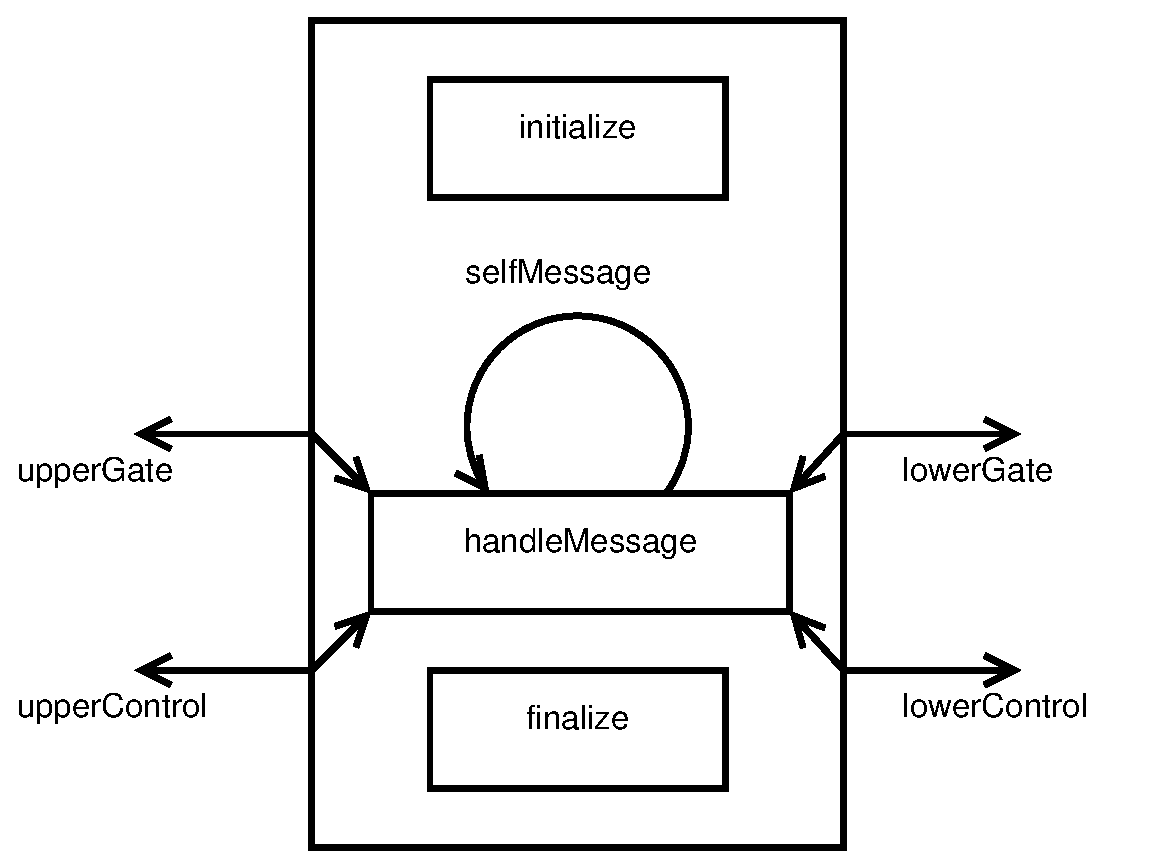
\includegraphics[width=0.5\textwidth]{omnetmodule.eps}
 \end{center}
 \caption{Basic \ac{OMNeT++} module structure}
 \label{fig:omnetmodule}
\end{figure}
 \item \textbf{sendDown/sendUp/sendControlDown/sendControlUp }These methods send a message from a module through the already commented gates.
 \item \textbf{scheduleAt - }This method schedules a self message in a certain time in the future. This is useful to programme timers or when a
message should be sent with a delay.
 \item \textbf{decapsMsg/encapsMsg - }Usually before a message is sent from one layer to another in the same device, it should be encapsulated or 
decapsulated. When this is done, instead of message, it is referred as packet. \textit{Packet} is a class which inherits from the class \textit{message}. It 
is also possible to define a custom packet (check \cite{manualomnet} for this).
\end{itemize}

These methods, and no others, were commented because they will be used many times during this work. For more information about \ac{OMNeT++}, 
please refer to the user manual \cite{manualomnet}.

\subsection{\ac{MiXiM} Framework}

The \ac{MiXiM} 2.0 framework provides \ac{OMNeT++} with many new modules. Among them, all the modules needed to work with 802.15.4 Standard. 
All these modules are build following \cite{IEEE802.15.4-2006}.

The basic structure of a node in \ac{MiXiM} is as shown in Figure \ref{fig:miximmodule}. This figure shows already some new modules added in
this work to the basic \ac{MiXiM} node. Depending on the kind of node, Computer, \ac{AN} or \ac{MN}, the \textit{.ned} files will load 
different modules to describe each behavior. These files should be also checked if a complete list of parameters is needed.

\begin{figure}[ht]
 \begin{center}
  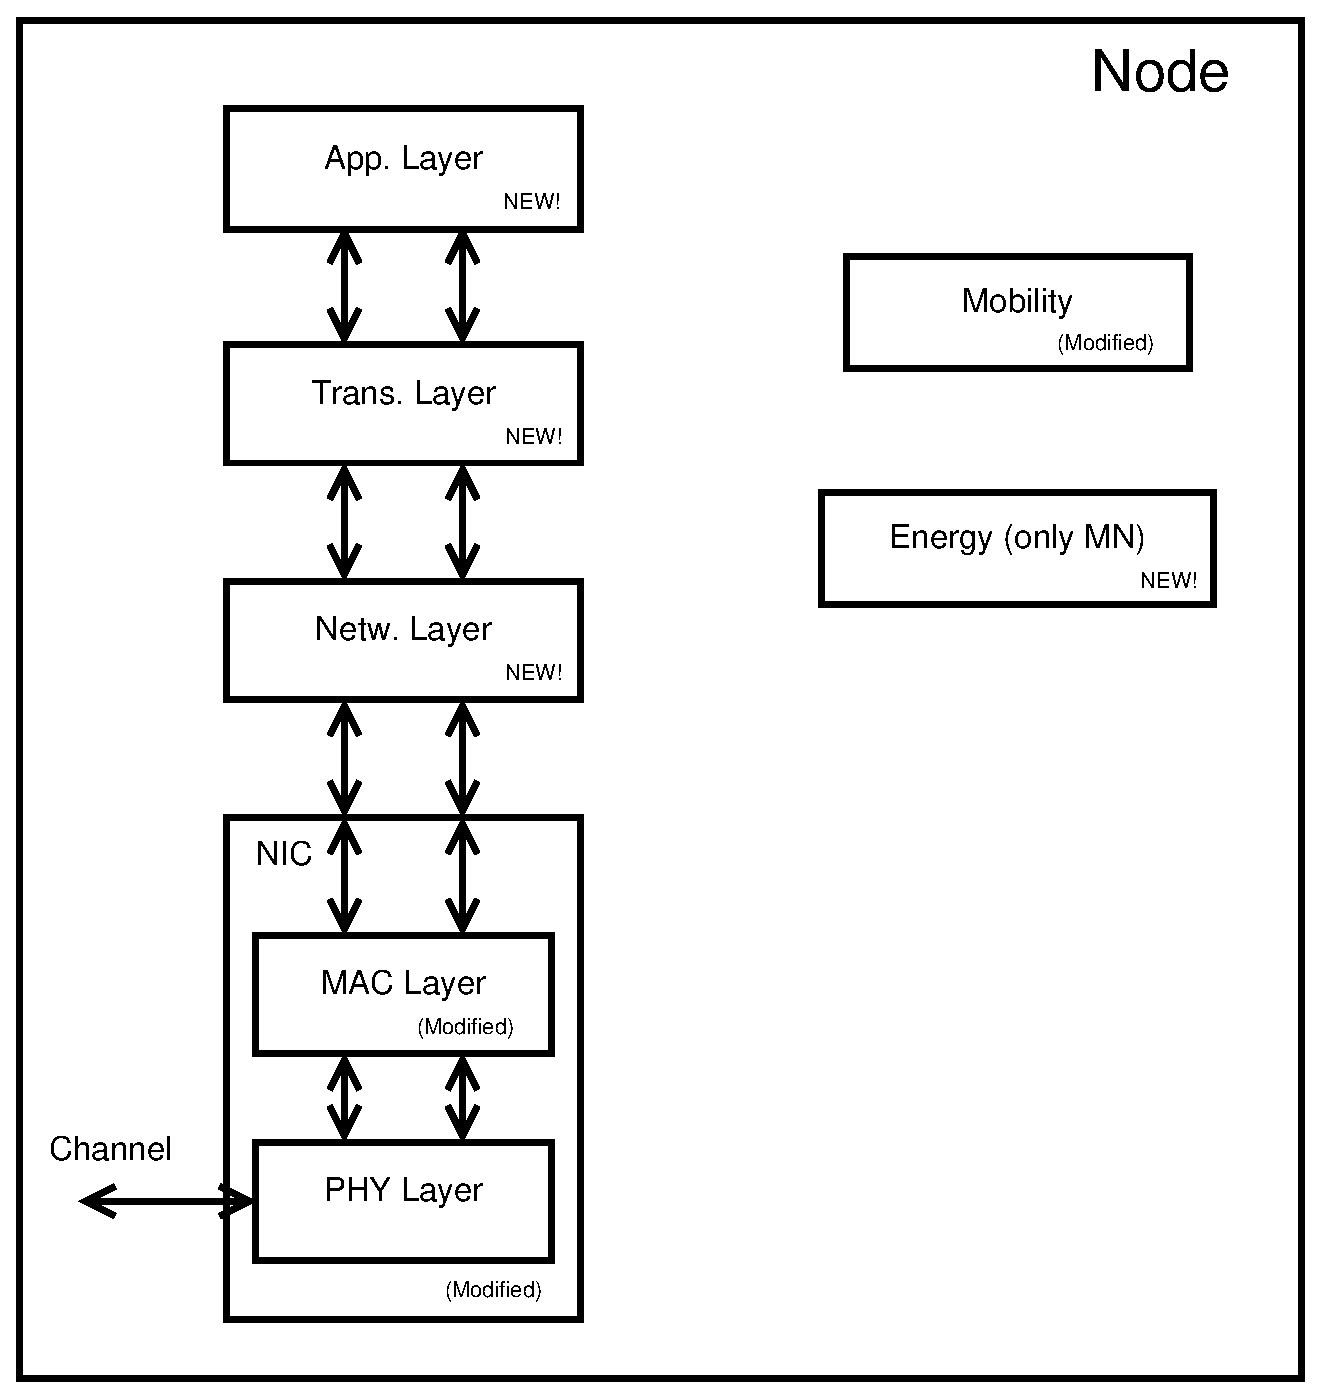
\includegraphics[width=0.8\textwidth]{miximmodule.eps}
 \end{center}
 \caption{Basic \ac{MiXiM} node structure}
 \label{fig:miximmodule}
\end{figure}

In this sub-section, only modified \ac{MiXiM} original modules will be commented, leaving the new implemented modules for the next sub-sections.

\subsubsection{New packet structure}
\label{sec:packetstructure}

In \ac{OMNeT++}, there are special files (\textit{.msg}), which define types of messages. When the project is compiled, a class is automatically 
generated from every \textit{.msg} file. \ac{MiXiM} contributes to \ac{OMNeT++} with many different message files. One of these files is the 
\textit{ApplPkt.msg}. This packet is generated in the Application Layer and encapsulated in every layer until it is transmitted into the 
air. For this purpose, this packet must include the following information which has not before:
\begin{itemize}
 \item \textit{realDestAddr} and \textit{realSrcAddr}. These values may be better understood with an example. When a \ac{MN} sends a report to the 
computer, the first step is sending the report to the selected \ac{AN}. This \ac{AN} will be the \textit{destAddr}, but the report is really intended
to go until the computer, who is the \textit{realDestAddr}. When this report arrives to the computer, to it, the \textit{srcAddr} is the 
address of the selected \ac{AN}, and the address of the \ac{MN} might be the \textit{realSrcAddr}.
 \item \textit{retransmisionCounterBO} and \textit{retransmisionCounterACK}. Whenever the \ac{MAC} Layer informs the Application Layer that a 
packet was dropped, the Application Layer checks if there still are more retransmissions available for this packet. The counter
\textit{retransmisionCounterBO} is used to check when a packet was dropped due to maximum number of Backoffs reached. \textit{retransmisionCounterACK} 
counter is used to check the case in which the packet was dropped because no \ac{ACK} was received. These counters are
increased by the Application Layer whenever a packet is retransmitted.
 \item \textit{CSMA}. This variable is a boolean. If it is true, indicates to the \ac{MAC} Layer that \ac{CSMA/CA} has to be disabled for 
this packet.
 \item \textit{askForRequest} and \textit{requestPacket}. These two flags are also booleans. When \textit{askForRequest} is true, it means
that \ac{MN} wants to notify the selected \ac{AN} that, in the next period, will be asked for data. When \textit{requestPacket} is true, it
means that \ac{MN} is requesting information to the selected \ac{AN}. These flags exist to help the selected \ac{AN} to know which kind of 
report it is receiving.
\end{itemize}

This packet structure is for simulation purposes only and has no relation with the real packet structure and, hence, with the size of the 
packet (\textit{bitLength} from \textit{cMessage} class) sent into the channel. Apart from Application Layer's packet, \ac{MAC} and 
\ac{PHY} Layer will add their own headers. From Figure \ref{fig:MACFrame} on page~\pageref{fig:MACFrame} and Figure \ref{fig:PPDU} on 
page~\pageref{fig:PPDU} is obtained that \ac{MAC} Layer header has 104 bits, and \ac{PHY} Layer header has 48 bits. This \ac{MAC} Layer's
header size, assumes both addresses as short addresses. But, in case a report has its origin or destination in a \ac{MN}, a long address 
must be used. This 6 bytes of difference between long and short addresses, will be compensated adding them to the Application Layer's packet size.

According to Application Layer, the following real packets can be distinguished:
\begin{itemize}
 \item \underline{Sync Packet}. Has 1 byte for the status, 4 bytes for the next phase time-stamp and $2 + 2 + 2$ bytes for \ac{AN} position. 
Hence, its size is 88 bits.
 
 \item \underline{Normal Report}. Reports the \acp{RSSI} listened during the former Sync Phases. It has 1 byte for the status and 2 bytes 
for each listened \ac{AN}. This kind of report only exists for \acp{MN} in modes 1 and 4. As the source address is a \ac{MN}, 6 bytes have to be added.
Hence, its size is $56 + 2\cdot X$ bits, where X is the number of \acp{AN} a Sync Packet has been listened to.

 \item \underline{\ac{MN} in mode 2 Report}. Reports the calculated positions by itself. It has 1 byte status and $2 + 2 + 2 = 6$ position 
bytes for each position calculated (maximum five). This report exists only for \acp{MN} in Mode 2. As the source address is a \ac{MN}, 6 bytes 
have to be added. Hence, its size is $56 + 6\cdot X$ bits, where X is the number of calculated positions to transmit.

 \item \underline{Ask Report}. Report or extra report with the ASK flag activated. In this case, 10 bytes are added to the report in which the
flag is activated. These 10 bytes represent the information needed by the selected \ac{AN} to know which data the \ac{MN} is asking for.

 \item \underline{Request}. Report or extra report with the Request flag activated. In this case, 1 byte is added to the report in which the
flag is activated. This byte tells which information was requested.

 \item \underline{\ac{MN}'s broadcast}. Broadcast packet sent by \acp{MN} in modes 3 and 4. It has 1 byte for the status and 1 byte information.
As the source address is a \ac{MN}, 6 bytes have to be added. Hence, its size is 64 bits.

 \item \underline{\ac{AN}'s answer to request}. Report sent by \acp{AN} when answering a \ac{MN}'s request. It has 1 byte status and 10 bytes info.
As the destination address is a \ac{MN}, 6 bytes have to be added. Hence, its size is 136 bits.

 \item \underline{Broadcasts collection packet}. Report sent by an \ac{AN} as collection of all broadcasts received from a \ac{MN} in mode 3 
or 4. It has 1 byte status, 2 bytes for \ac{RSSI} info and 6 bytes for showing to which \ac{MN} the \ac{RSSI} belongs to. Hence, its size is 72 bits.
\end{itemize}

\subsubsection{Connection Manager}

Apart from the node structure modules, there is a central module in \ac{MiXiM}, called \textit{connectionManager}. This module is in charge of connecting
all nodes at a reachable distance. It keeps a list of all nodes and it is called every time a node changes its position. Then, \textit{ConnectionManager} 
updates the position in the list and recalculates all connections. The maximum distance in which two nodes could still reach each other is 
calculated using the transmit power and sensitivity, both defined in \textit{omnetpp.ini}.

Each element from the node list is an object of the class \textit{NicEntry}. This class stores, among many other data, the coordinates of the
position of the node. This class was modified to store also the following data:

\begin{itemize}
 \item \underline{Module Type}. It stores, in the variable \textit{moduleType}, the node type this \ac{NIC} belongs to. The values could be 1 for \ac{AN}, 
2 for \ac{MN} and 3 for Computer. Its value is assigned when the node is being initialized. Defining this variable here, it can be read from all modules in the 
network. This is useful to make lists of the different kinds of nodes.

 \item \underline{Slot Information}. Through the variables \textit{transmisionSlot} and \textit{numSlots}, the \ac{AN} knows which slots of the 
\textit{numTotalSlots} are the ones reserved to it to transmit. All these three variables are assigned by the Computer in its \textit{initialize} method.
\end{itemize}

\subsubsection{Mobility module modifications}

The mobility module is the responsible of the node's positions. It is the one who assigns the initial position to the nodes and it is also the one
used whenever a node wants to be moved. This module's functionality is described in class \textit{BaseMobility}. As the position of the nodes is needed,
this class is also linked with the \textit{NicEntry} class. Unlike \textit{connectionManager}, this is not a general module and each node has its own
mobility module as it can be seen in Figure \ref{fig:miximmodule}.

During \textit{initialize} method in \textit{BaseMobility}, all node's initial positions are assigned according to the values given in the file
\textit{omnetpp.ini}. A different value for each coordinate (X, Y, Z) must be given and all of them must be inside the playground area (defined also
in \textit{omnetpp.ini}). When, instead of a fixed value for the position, a ``-1'' is given, node will get a random position. The modifications done to
this class refer precisely to the node's initial position assignment.

\begin{itemize}
 \item \underline{Uniform random distribution}. It was already seen that, assigning ``-1'' as value for a node's coordinate, this coordinate will be 
randomly assigned. But, if all coordinates are ``-1'', a new peace of code at \textit{stage} = 2 during \textit{initialize} method is executed. This 
code distributes \acp{AN} and \acp{MN} uniformly and randomly in the playground according to \textit{minimumDistanceAnchor} and 
\textit{minimumDistanceNode} parameter respectively. These two variables represent, as their names show, the minimum distance to leave among \acp{AN} 
and the minimum distance to leave among \acp{MN}.

 \item \underline{Grid distribution}. When ``-2'' is assigned to all \ac{AN}'s coordinate values in \textit{omnetpp.ini}, all \acp{AN} will be 
distributed all over the playground forming a grid. The dimensions of the grid will depend on the number of \acp{AN}, resulting, for example, for 25 
\acp{AN} a 5 x 5 grid. This grid distribution will be done at \textit{stage} = 0 during \textit{initialize} method.
\end{itemize}

\subsubsection{\ac{MAC} Layer modifications}
\label{sec:macmodifications}

\ac{MAC} Layer for 802.15.4 in \ac{MiXiM} is defined by the \textit{csma} class. This class works as a \ac{FSM} whose diagram is as shown in Figure 
\ref{fig:csmaFSM}.

\begin{figure}[ht]
 \begin{center}
  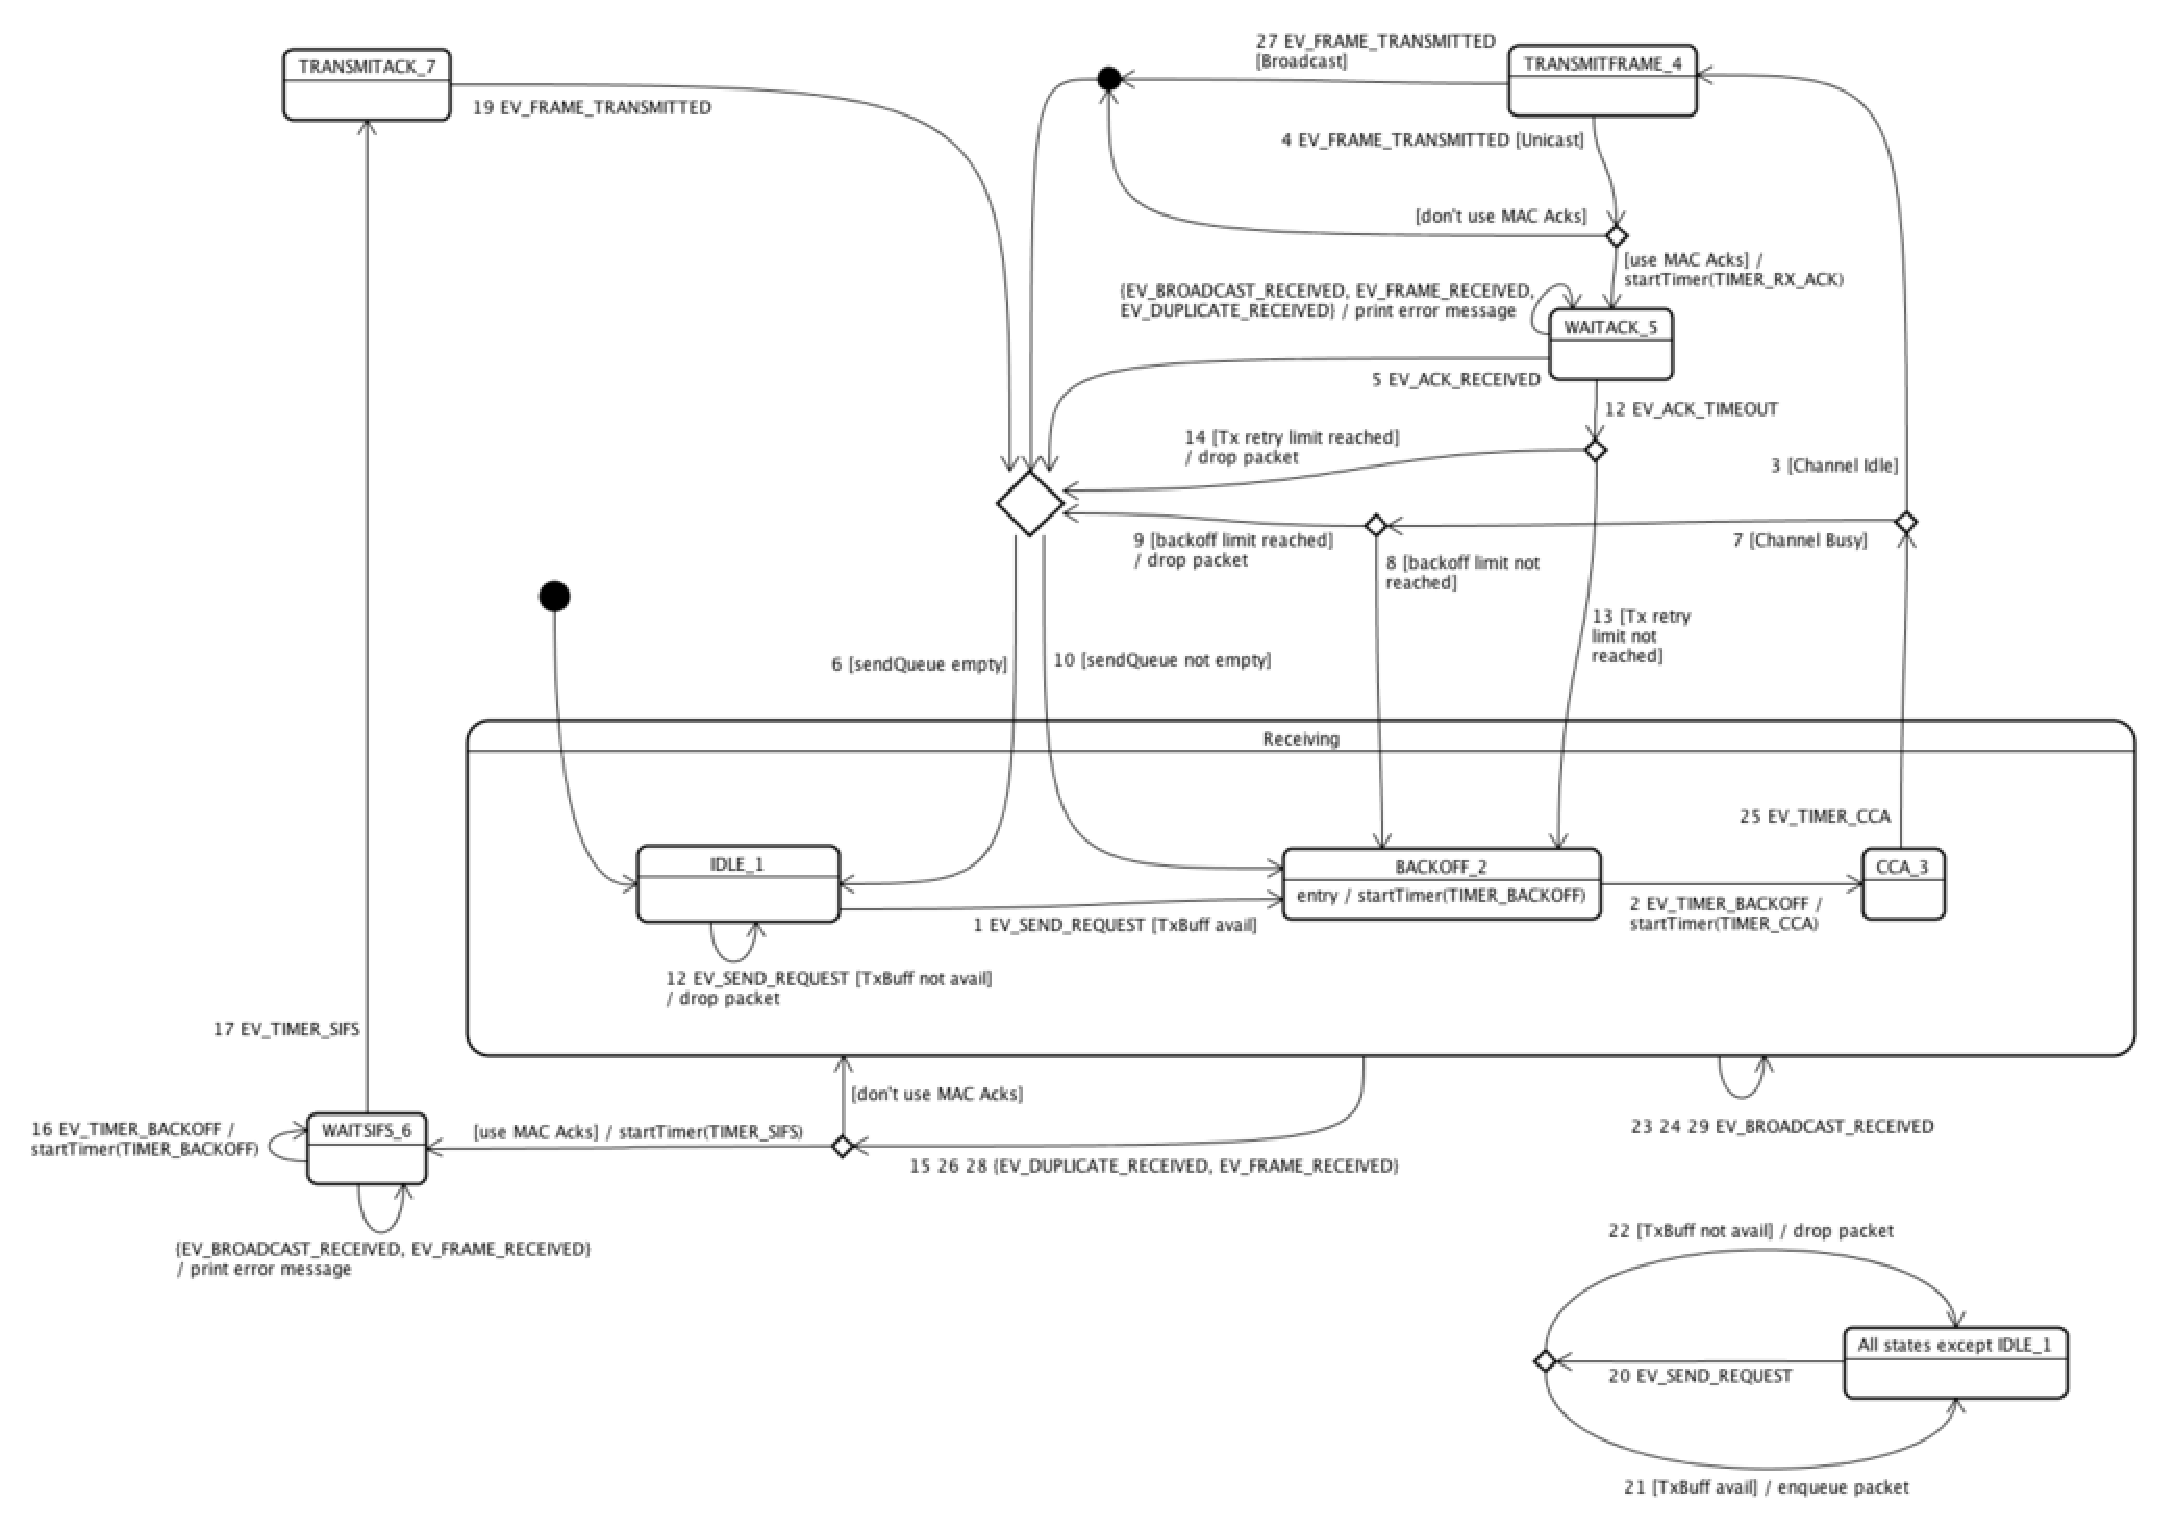
\includegraphics[width=1\textwidth]{csmaFSM.eps}
 \end{center}
 \caption{\ac{MiXiM}'s 802.15.4 \ac{MAC} Layer \ac{FSM} diagram \cite{MiXiM}}
 \label{fig:csmaFSM}
\end{figure}

Modifications done to this class are:

\begin{itemize}
 \item \underline{\ac{CSMA/CA} disabling possibility}. During the method \textit{updateStatusIdle} and whenever there is a packet in \ac{MAC} queue to
be transmitted, the first Backoff time would be calculated. In case the \ac{CSMA/CA} is deactivated, instead of calculating the first Backoff
time and scheduling the \ac{CCA} at this time, \ac{CCA} will be scheduled after \ac{SIFS} seconds (to assure Radio is in Rx state). If after the
\ac{CCA} the channel is busy, the packet must be directly discarded instead of calculating a second Backoff time. That is why the \ac{NB} is 
set to the maximum number of retries. 

 \item \underline{Protocol phases end control}. A way to control in which phase the node is was added. This control is started during the
\textit{initialize} method at stage 4 and it is rescheduled for every phase from method \textit{handleSelfMsg}. This control makes the 
\ac{MAC} Layer, at the beginning of every phase, check if the \ac{MAC} queue has elements from previous phase, in which case are erased and 
the number of elements recorded, to have it as a result when the \textit{finish} method is called.

Before the end of every phase, a \textit{guardTransmitTime} time is left. When \ac{MAC} Layer tries to send the next packet into the queue, if the end of 
the first Backoff time goes beyond the guard time, the packet is not scheduled but erased. The erased packets number is also recorded
to be extracted as a result. This guard time in this work is 10 ms. It is this long to be protected even against the biggest packets during the 
simulation.

 \item \underline{Energy management}. In \ac{MiXiM}, although \ac{PHY} Layer has a SLEEP state, it is never used. This work makes \acp{MN}
go to sleep whenever they are able to. As this matter will be treated in Section \ref{sec:frameworkdevelopment} (\nameref{sec:frameworkdevelopment})
in a deeper way, here it would be just commented that, whenever a \ac{MAC} state or a \ac{PHY} state gets changed in \textit{csma} class, another
class called \textit{energy} has to be warned.

 \item \underline{New control messages}. Before the modifications, \textit{csma} class informed upper layers whenever a sent report received an
\ac{ACK}. Now, it informs also when broadcasts and \acp{ACK} were successfully sent to the channel. This class was also modified to 
report when a packet is dropped due to maximum number of Backoff retries, to maximum number of ``no \ac{ACK} received`` retries or when
\ac{MAC} Queue is full. Before, it was only informing about packet dropping, but without any reason. All these control messages will be treated 
in the Application Layer and will be studied in following sections.
\end{itemize}

For a deeper view of \ac{MiXiM}'s \ac{MAC} Layer, a look up at \cite{MiXiM} and a deep view into the source code together with the diagram in Figure 
\ref{fig:csmaFSM} are recommended.


\section{Sync Phase study development}

Before constructing all the protocol framework, it had to be decided if during the Sync Phase the \acp{AN} would transmit their broadcasts 
synchronized in slots or randomly. For this purpose, a special and small framework was done, where just a simple Application Layer was added to 
the nodes. As this was just a temporary Application Layer, only the main aspects of it will be given.

\textit{Decider802154Narrow} class was modified to disable errors caused by noise and random errors due to the channel. These features were 
enabled again for the protocol framework development. This way whenever there is a fail, it can be known that it is due to simultaneous \ac{CCA}
or Hidden Terminal Problem.

\subsection{\ac{MN}}

\ac{MN} is the one receiving the broadcasts sent by the \acp{AN}. The only task for the \ac{MN} is, whenever it receives a broadcast, to
store as a variable information about when and from which \ac{AN} the broadcast came. This way the performance could be analyzed later.

\subsection{Computer}

Computer does not really participate in the packet exchange, but it calculates the slot distribution among the \acp{AN} for the slotted case. 
Slot calculation is done according to the algorithm showed in Section \ref{subsec:slottedsyncphase} (\nameref{subsec:slottedsyncphase}). Computer 
also calculates the length of the different phases in the period. This length information is needed when packets are randomly transmitted 
during Sync Phase to compare with the slotted case, otherwise the maximum time to transmit will not be known. Slots calculation is done at
\textit{stage} 3 during \textit{initialize} method in \textit{ComputerAppLayer} class.

\subsection{\ac{AN}}

\acp{AN} are the responsibles to send the broadcasts to be detected by the \ac{MN}. Depending on the mode (slotted or random) the 
behavior changes:
\begin{itemize}
 \item \underline{Random}. The first random broadcast gets scheduled at \textit{stage} 4 during \textit{initialize} method in \textit{AnchorAppLayer}
class. It gets scheduled a random time after starting the simulation. This random time has a maximum value defined in 
\textit{syncFirstMaxRandomTime}. Every time a message is sent, the next one is scheduled in a random time from this moment. This random 
time has also a maximum, but this time defined in \textit{syncRestMaxRandomTimes}. To make simulation easier, these two variables are going to get
always the same values.

The retransmission is done in \textit{handleLowerControl}
method whenever a broadcast was successfully sent in the channel and if the already sent broadcasts number is smaller than 
\textit{syncPacketsPerSyncPhase}. If on the other hand, the broadcast was not successfully sent into the channel, it is retransmitted, recording
it for the results.
 \item \underline{Slotted}. At \textit{stage} 4 during \textit{initialize} method, the first packet in the first slot is scheduled. This is done
in \textit{stage} 4 and not before, because all slot information is calculated by the computer in \textit{stage} 3. The next slotted packets to
send are scheduled during the \textit{handleSelfMsg} method. In this mode, the \textit{handleLowerControl} method has no functionality as all 
packets would be sent into the channel without problems. The number of slots per \ac{AN} during a Sync Phase, will be defined also by the variable 
\textit{syncPacketsPerSyncPhase}.
\end{itemize}


\section{Framework development}
\label{sec:frameworkdevelopment}

Apart from the modules already commented, the only ones yet to be introduced are the relatives to the node structure. These are the ones marked
with ''NEW$!$`` in Figure \ref{fig:miximmodule}. Due to their similarity among types of nodes and their simplicity, the modules 
\textit{Energy}, Transport Layer and Network Layer are going to be explained all together. However, the Application Layers are going to be 
explained separately for \acp{AN}, \acp{MN} and Computer.

\subsection{Energy module}

Although this module is available for all types of nodes, it will be used just for \acp{MN}, as these are the nodes in which the energy 
consumption is important. Whenever a \ac{MAC} or \ac{PHY} state is 
changed in \ac{MAC} or Application Layers, this module's main method will be called (\textit{updateStateStatus}). This class 
(\textit{EnergyConsumption}) will also \textit{initialize} with lots of default values and will \textit{finish} saving many different 
time values and calculating energy values to be studied later on.

In \ac{MiXiM}, \ac{PHY} Layer has no IDLE state. Hence, this work used the \ac{Rx} state to represent both \ac{Rx} and IDLE states. But this is
not 100\% correct, because the consumed energy in both states is not the same. That is why this module was created implementing its own state machine,
with the states SLEEP, \ac{Rx}, \ac{Tx} and IDLE. The transition among all the states can be observed in Figure \ref{fig:statesDiagramEnergy}. 
Inside the circles, with a bigger font, it is said the state of the \textit{Energy} module and with a smaller font, the equivalent \ac{MAC} 
states.

\begin{figure}[ht]
 \begin{center}
  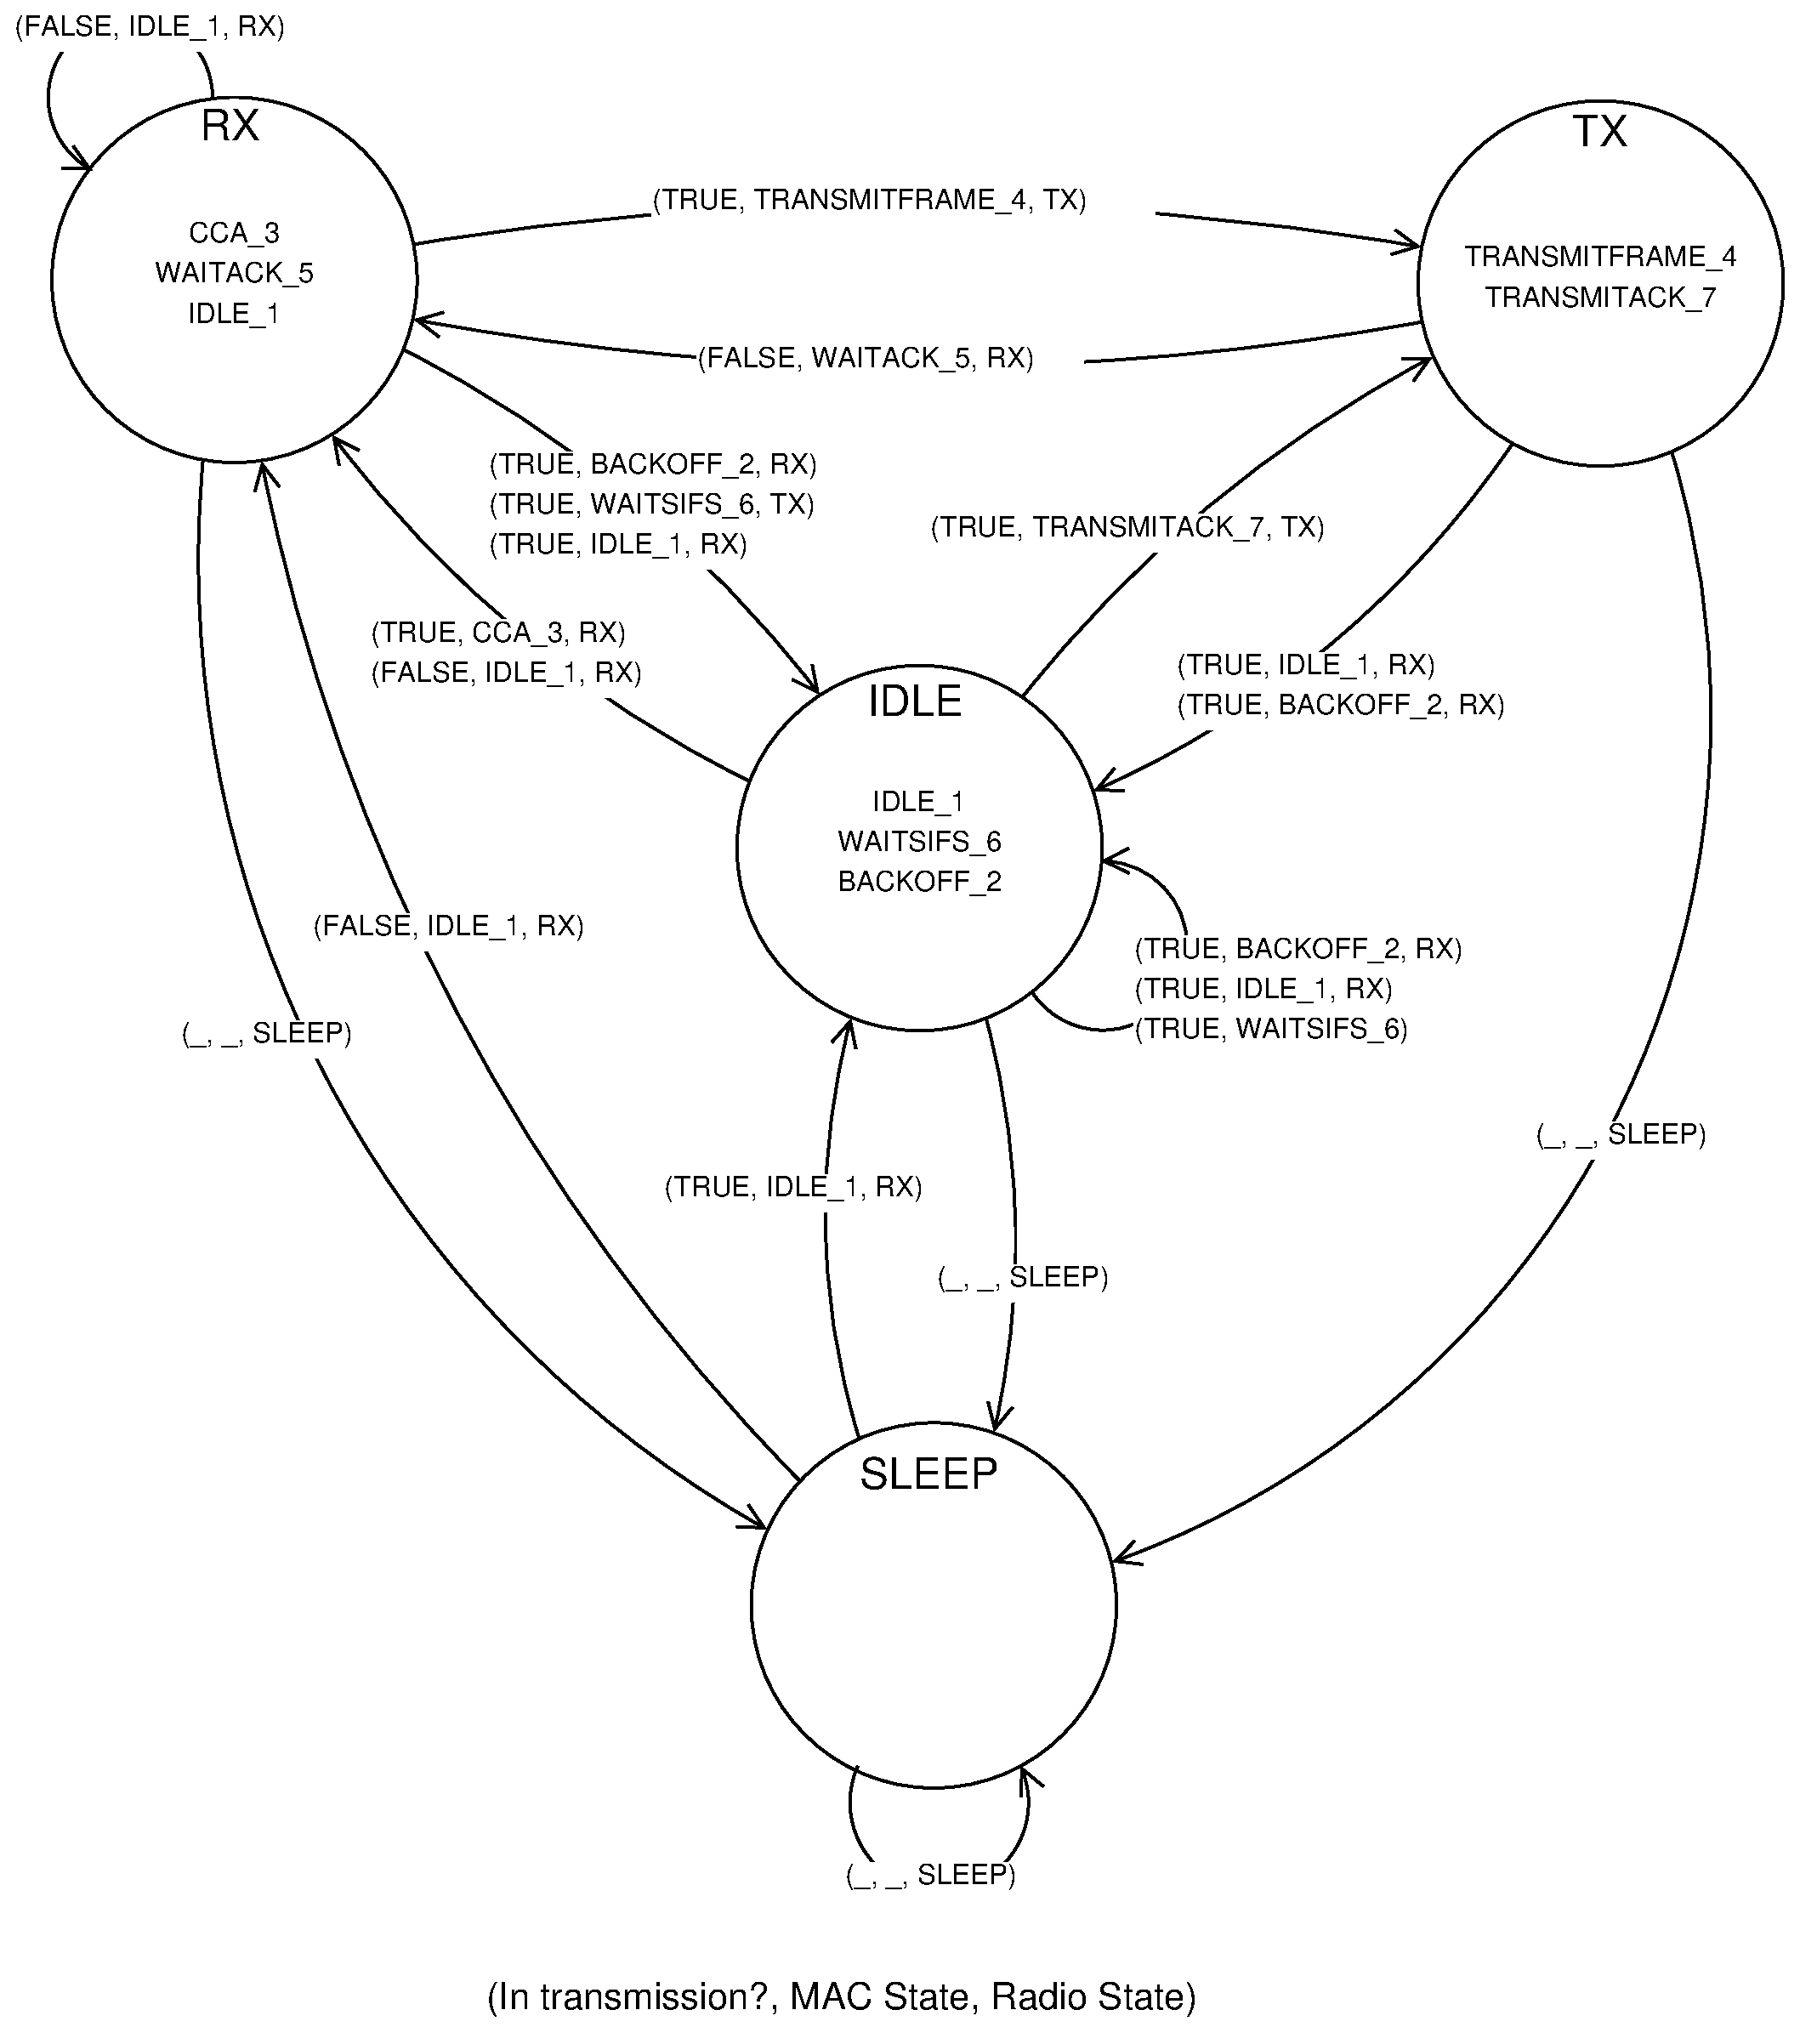
\includegraphics[width=0.8\textwidth]{statesDiagramEnergy.eps}
 \end{center}
 \caption{\textit{Energy}'s \ac{FSM} diagram}
 \label{fig:statesDiagramEnergy}
\end{figure}

Whenever there is a transition between two states, the three values between brackets on the figure (A, B, C) are passed as argument of the 
\textit{updateStateStatus} method. If one of these values in the figure takes the \_ value, the value sent in this position is ignored.

First value (A, \_, \_) is a boolean indicating true if the \ac{MN} is in a packet transmission process or false if it is in IDLE or packet 
reception process. This flag might be important in some cases to differentiate when \ac{PHY} state \ac{Rx} is really being used as \ac{Rx} or as
IDLE.

Second value (\_, B, \_) indicates the \ac{MAC} state the \ac{MAC} Layer is changing to. Some times it is necessary to change \ac{PHY} Layer state
without modifying the \ac{MAC} state from the Application Layer. This Layer has no access to know in which state the \ac{MAC} Layer is. This is
why, when \ac{MAC} state does not want to be changed, the total number of \ac{MAC} states must be given.

Third value (\_, \_, C) indicates the \ac{PHY} state the Radio is changing to. For the same reason as before, the total number of \ac{PHY} states
may be given.

The main functionalities of \textit{updateStateStatus} method are:
\begin{itemize}
 \item Calculate and change the new Energy State according to the previous state and the given arguments, following the diagram in Figure
\ref{fig:statesDiagramEnergy}.
 \item Calculate through time-stamps, the total time that \acp{MN} were in each state, as well as how much time was spent on all the different
transitions.
 \item Calculate the time the microprocessor spent calculating a \ac{MN} position (\ac{MN} in Mode 2). During this time, transceiver
state and, hence, energy state, are in SLEEP, but the microprocessor is working, spending an energy that should be taken into account.
\end{itemize}

\subsection{Transport Layer}

Transport Layer from Computer, \acp{AN} and \acp{MN} does not really do anything else than forwarding messages and control messages coming from 
Network Layer to Applications Layer and vice versa. This Layer was built to have a main structure available for a future work, when 
aggregation and segmentation were needed as an idea to reduce traffic in the network. The three classes are \textit{ComputerTransLayer},
\textit{AnchorTransLayer} and \textit{NodeTransLayer} respectively.

\subsection{Network Layer}

As it was commented in Chapter \ref{chap:802154standard} (\nameref{chap:802154standard}), the topology of the network selected for this work
is the tree topology. In this topology all \acp{AN} can communicate only with their parents or children. On the top of this topology, there is 
the computer.

A complicate routing protocol would be out of the scope of this project. That is why a network where all \acp{AN} do not change their positions 
in every simulation is needed, in concrete a grid topology was chosen. The reasons to choose a grid topology were its simplicity and the fact of 
being a standard network in which, as found in literature, many protocols are tested \cite{GridNetworks}. For our work, an scenario like the one 
in Figure \ref{fig:finalscenario} will be used in Chapter \ref{chap:simulationandresults} (\nameref{chap:802154standard}).

Assuming that the \acp{AN} are fixed and situated like shown in Figure \ref{fig:finalscenario}, the tree topology displayed in Figure 
\ref{fig:routetree} is obtained. With this topology, a routing matrix could be easily extracted and stored in the nodes. This way nodes 
are able to know which next hop the packet should make to reach its final destination.

\begin{figure}[ht]
 \begin{center}
  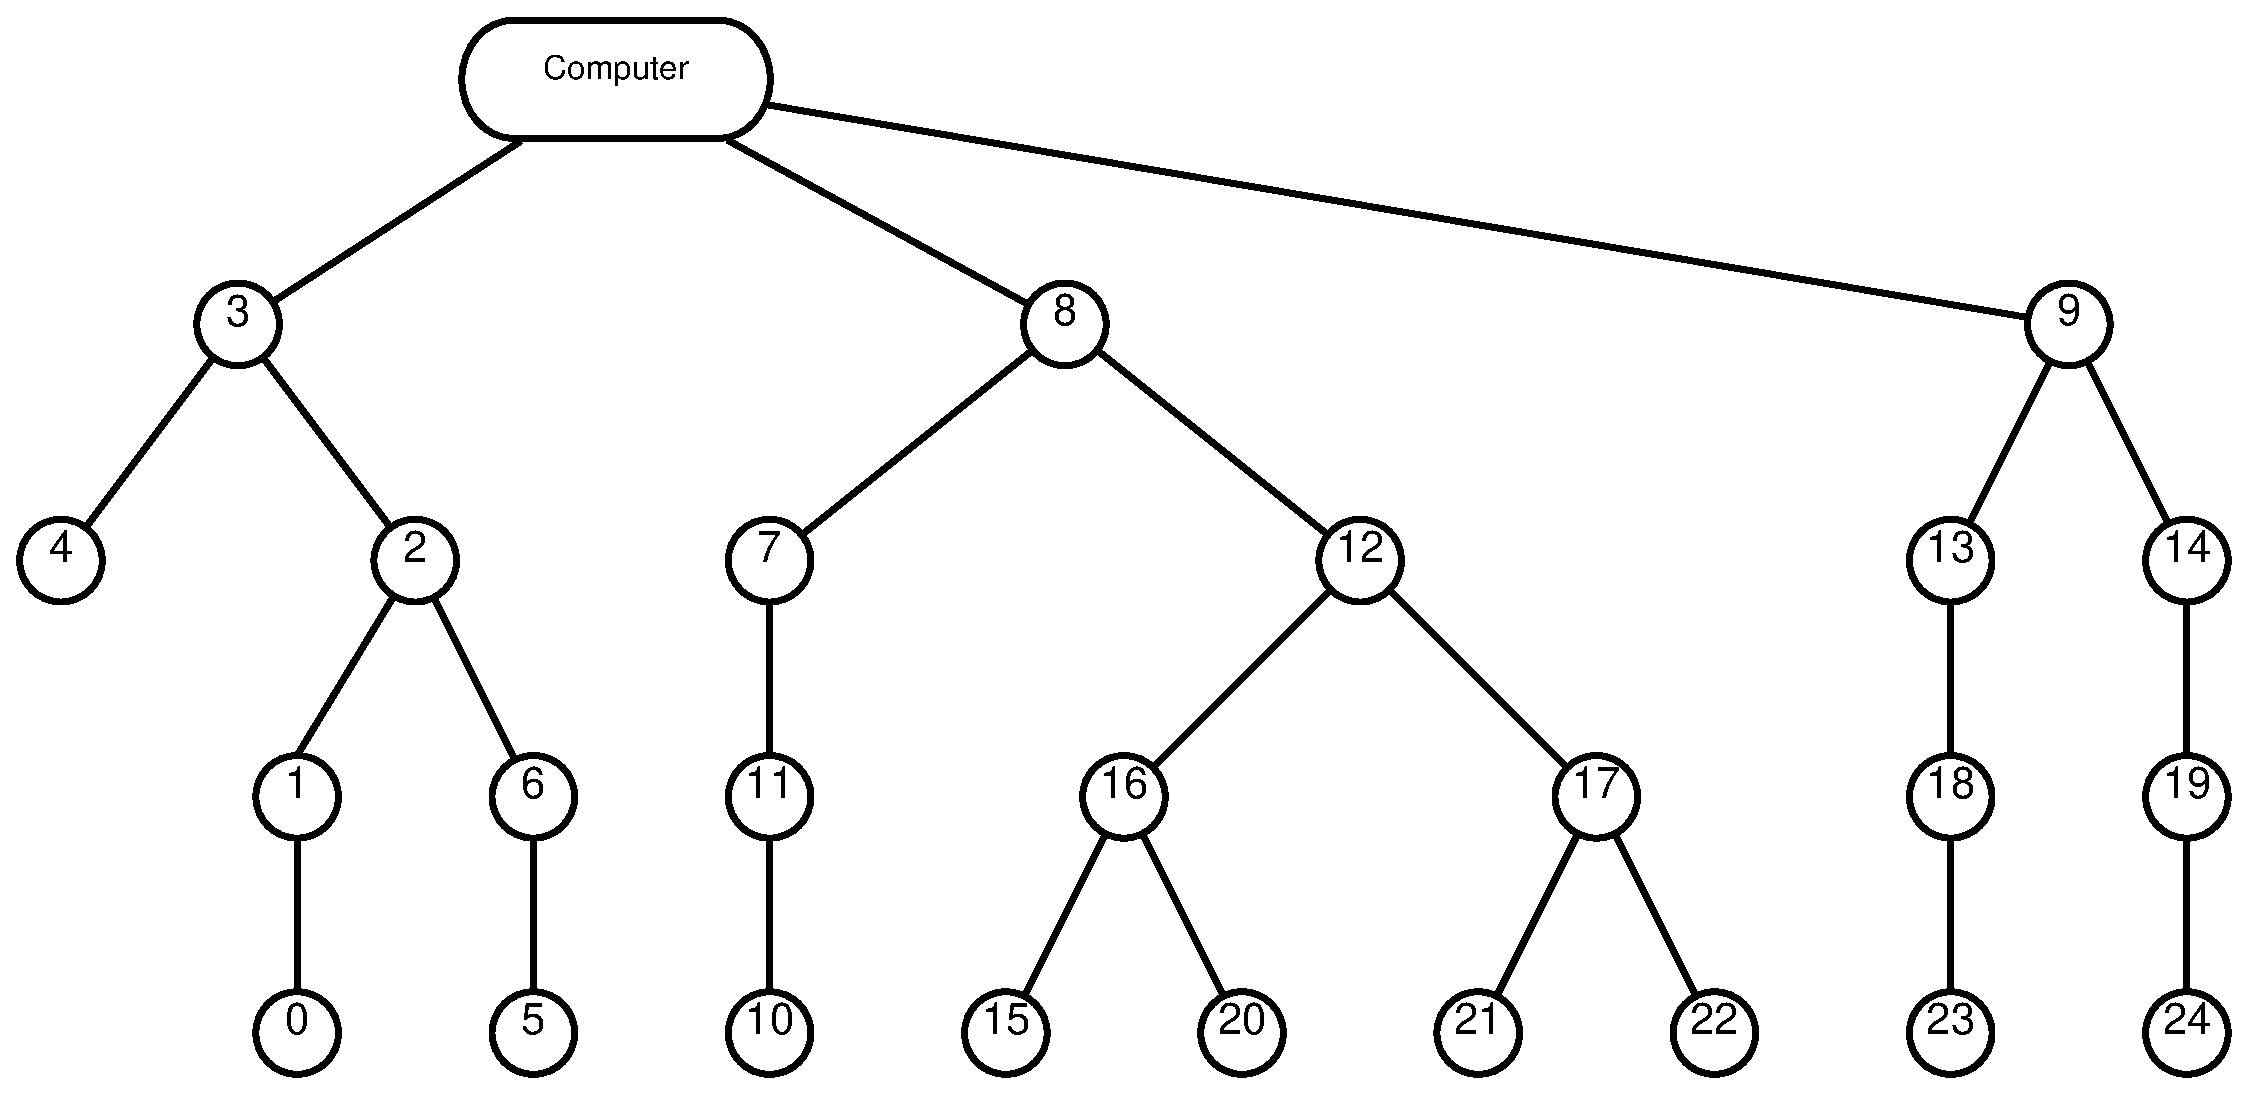
\includegraphics[width=0.8\textwidth]{routetree.eps}
 \end{center}
 \caption{Routing Tree Topology}
 \label{fig:routetree}
\end{figure}

Network Layer is present in the Computer, \acp{AN} and \acp{MN}, being the classes describing its functionality \textit{ComputerNetLayer},
\textit{AnchorNetLayer} and \textit{NodeNetLayer} respectively. All these classes have the same structure and their main methods are the following:
\begin{itemize}
 \item \textit{handleLowerControl}: this method receives a control message from \ac{MAC} Layer through Transport Layer and redirects it to the
Application Layer.

 \item \textit{handleUpperControl}: this method receives a control message from Application Layer and redirects it to the \ac{MAC} Layer through
Transport Layer.

 \item \textit{handleLowerMsg}: this method receives a message from \ac{MAC} Layer through Transport Layer and, after decapsulating it, sends it
to the Application Layer.

 \item \textit{handleUpperMsg}: this method receives a message from Application Layer and, after encapsulating it, sends it to the \ac{MAC}
Layer through Transport Layer.

 \item \textit{encapsMsg}: this method adds (or encapsulates) a header to the Application message with the address of the next hop. This 
header will be, however, 0 bit long because, although the address is calculated here, it is only encapsulated to provide it to the \ac{MAC} Layer.
\ac{MAC} Layer will include it in its header, taking there the necessary bits to be transmitted. This method will also attach information 
indicating if \ac{CSMA/CA} must be deactivated or not. This info will be interpreted in the \ac{MAC} Layer.

The destination address will be calculated differently depending on the case. When broadcasting, the value ''-1`` is assigned. This is 
interpreted by the \ac{MAC} Layer to send a broadcast. When the node is a \ac{MN}, as it does not need to route the packet because it 
can communicate only with its selected \ac{AN}, the next hop address will be the one of its \ac{AN}. However, when the node is an \ac{AN}
or the Computer, using the source and destination address, the next hop address is obtained from the routing matrix. For this work, the 
destination matrix corresponds to the one on Table \ref{tab:routingmatrix}.

 \item \textit{decapsMsg}: this method removes (or decapsulates) the header added by the Network Layer of the sending node to recover the 
original Application message. It also attaches the \ac{RSSI} and Bit Error Rate information provided by the \ac{MAC} Layer about the 
reception of this packet. Thanks to this attachment, this information will be available to the Application Layer.
\end{itemize}

\begin{table}[ht]\tiny
 \begin{center}
  \begin{tabular}{|c|p{0.1cm}|p{0.1cm}|p{0.1cm}|p{0.1cm}|p{0.1cm}|p{0.1cm}|p{0.1cm}|p{0.1cm}|p{0.1cm}|p{0.1cm}|p{0.1cm}|p{0.1cm}|p{0.1cm}|p{0.1cm}|p{0.1cm}|p{0.1cm}|p{0.1cm}|p{0.1cm}|p{0.1cm}|p{0.1cm}|p{0.1cm}|p{0.1cm}|p{0.1cm}|p{0.1cm}|p{0.1cm}|p{0.1cm}|}
   %\noalign{\vspace*{0.5cm}}
   \hline
   \textbf{\acp{AN}} & \textbf{0} & \textbf{1} & \textbf{2} & \textbf{3} & \textbf{4} & \textbf{5} & \textbf{6} & \textbf{7} & \textbf{8} & 
   \textbf{9} & \textbf{10} & \textbf{11} & \textbf{12} & \textbf{13} & \textbf{14} & \textbf{15} & \textbf{16} & \textbf{17} & \textbf{18} & 
   \textbf{19} & \textbf{20} & \textbf{21} & \textbf{22} & \textbf{23} & \textbf{24} & \textbf{C} \\
   \hline
   \textbf{0} & 0 & 1 & 1 & 1 & 1 & 1 & 1 & 1 & 1 & 1 & 1 & 1 & 1 & 1 & 1 & 1 & 1 & 1 & 1 & 1 & 1 & 1 & 1 & 1 & 1 & 1 \\
   \hline
   \textbf{1} & 0 & 1 & 2 & 2 & 2 & 2 & 2 & 2 & 2 & 2 & 2 & 2 & 2 & 2 & 2 & 2 & 2 & 2 & 2 & 2 & 2 & 2 & 2 & 2 & 2 & 2 \\
   \hline
   \textbf{2} & 1 & 1 & 2 & 3 & 3 & 6 & 6 & 3 & 3 & 3 & 3 & 3 & 3 & 3 & 3 & 3 & 3 & 3 & 3 & 3 & 3 & 3 & 3 & 3 & 3 & 3 \\
   \hline
   \textbf{3} & 2 & 2 & 2 & 3 & 4 & 2 & 2 & C & C & C & C & C & C & C & C & C & C & C & C & C & C & C & C & C & C & C \\
   \hline
   \textbf{4} & 3 & 3 & 3 & 3 & 4 & 3 & 3 & 3 & 3 & 3 & 3 & 3 & 3 & 3 & 3 & 3 & 3 & 3 & 3 & 3 & 3 & 3 & 3 & 3 & 3 & 3 \\
   \hline
   \textbf{5} & 6 & 6 & 6 & 6 & 6 & 5 & 6 & 6 & 6 & 6 & 6 & 6 & 6 & 6 & 6 & 6 & 6 & 6 & 6 & 6 & 6 & 6 & 6 & 6 & 6 & 6 \\
   \hline
   \textbf{6} & 2 & 2 & 2 & 2 & 2 & 5 & 6 & 2 & 2 & 2 & 2 & 2 & 2 & 2 & 2 & 2 & 2 & 2 & 2 & 2 & 2 & 2 & 2 & 2 & 2 & 2 \\
   \hline
   \textbf{7} & 8 & 8 & 8 & 8 & 8 & 8 & 8 & 7 & 8 & 8 & 11 & 11 & 8 & 8 & 8 & 8 & 8 & 8 & 8 & 8 & 8 & 8 & 8 & 8 & 8 & 8 \\
   \hline
   \textbf{8} & C & C & C & C & C & C & C & 7 & 8 & C & 7 & 7 & 12 & C & C & 12 & 12 & 12 & C & C & 12 & 12 & 12 & C & C & C \\
   \hline
   \textbf{9} & C & C & C & C & C & C & C & C & C & 9 & C & C & C & 13 & 14 & C & C & C & 13 & 14 & C & C & C & 13 & 14 & C \\
   \hline
   \textbf{10} & 11 & 11 & 11 & 11 & 11 & 11 & 11 & 11 & 11 & 11 & 10 & 11 & 11 & 11 & 11 & 11 & 11 & 11 & 11 & 11 & 11 & 11 & 11 & 11 & 11 & 11 \\
   \hline
   \textbf{11} & 7 & 7 & 7 & 7 & 7 & 7 & 7 & 7 & 7 & 7 & 10 & 11 & 7 & 7 & 7 & 7 & 7 & 7 & 7 & 7 & 7 & 7 & 7 & 7 & 7 & 7 \\
   \hline
   \textbf{12} & 8 & 8 & 8 & 8 & 8 & 8 & 8 & 8 & 8 & 8 & 8 & 8 & 12 & 8 & 8 & 16 & 16 & 17 & 8 & 8 & 16 & 17 & 17 & 8 & 8 & 8 \\
   \hline
   \textbf{13} & 9 & 9 & 9 & 9 & 9 & 9 & 9 & 9 & 9 & 9 & 9 & 9 & 9 & 13 & 9 & 9 & 9 & 9 & 18 & 9 & 9 & 9 & 9 & 18 & 9 & 9 \\
   \hline
   \textbf{14} & 9 & 9 & 9 & 9 & 9 & 9 & 9 & 9 & 9 & 9 & 9 & 9 & 9 & 9 & 14 & 9 & 9 & 9 & 9 & 19 & 9 & 9 & 9 & 9 & 19 & 9 \\
   \hline
   \textbf{15} & 16 & 16 & 16 & 16 & 16 & 16 & 16 & 16 & 16 & 16 & 16 & 16 & 16 & 16 & 16 & 15 & 16 & 16 & 16 & 16 & 16 & 16 & 16 & 16 & 16 & 16 \\
   \hline
   \textbf{16} & 12 & 12 & 12 & 12 & 12 & 12 & 12 & 12 & 12 & 12 & 12 & 12 & 12 & 12 & 12 & 15 & 16 & 12 & 12 & 12 & 20 & 12 & 12 & 12 & 12 & 12 \\
   \hline
   \textbf{17} & 12 & 12 & 12 & 12 & 12 & 12 & 12 & 12 & 12 & 12 & 12 & 12 & 12 & 12 & 12 & 12 & 12 & 17 & 12 & 12 & 12 & 21 & 22 & 12 & 12 & 12 \\
   \hline
   \textbf{18} & 13 & 13 & 13 & 13 & 13 & 13 & 13 & 13 & 13 & 13 & 13 & 13 & 13 & 13 & 13 & 13 & 13 & 13 & 18 & 13 & 13 & 13 & 13 & 23 & 13 & 13 \\
   \hline
   \textbf{19} & 14 & 14 & 14 & 14 & 14 & 14 & 14 & 14 & 14 & 14 & 14 & 14 & 14 & 14 & 14 & 14 & 14 & 14 & 14 & 19 & 14 & 14 & 14 & 14 & 24 & 14 \\
   \hline
   \textbf{20} & 16 & 16 & 16 & 16 & 16 & 16 & 16 & 16 & 16 & 16 & 16 & 16 & 16 & 16 & 16 & 16 & 16 & 16 & 16 & 16 & 20 & 16 & 16 & 16 & 16 & 16 \\
   \hline
   \textbf{21} & 17 & 17 & 17 & 17 & 17 & 17 & 17 & 17 & 17 & 17 & 17 & 17 & 17 & 17 & 17 & 17 & 17 & 17 & 17 & 17 & 17 & 21 & 17 & 17 & 17 & 17 \\
   \hline
   \textbf{22} & 17 & 17 & 17 & 17 & 17 & 17 & 17 & 17 & 17 & 17 & 17 & 17 & 17 & 17 & 17 & 17 & 17 & 17 & 17 & 17 & 17 & 17 & 22 & 17 & 17 & 17 \\
   \hline
   \textbf{23} & 18 & 18 & 18 & 18 & 18 & 18 & 18 & 18 & 18 & 18 & 18 & 18 & 18 & 18 & 18 & 18 & 18 & 18 & 18 & 18 & 18 & 18 & 18 & 23 & 18 & 18 \\
   \hline
   \textbf{24} & 19 & 19 & 19 & 19 & 19 & 19 & 19 & 19 & 19 & 19 & 19 & 19 & 19 & 19 & 19 & 19 & 19 & 19 & 19 & 19 & 19 & 19 & 19 & 19 & 24 & 19 \\
   \hline
   \textbf{C} & 3 & 3 & 3 & 3 & 3 & 3 & 3 & 8 & 8 & 9 & 8 & 8 & 8 & 9 & 9 & 8 & 8 & 8 & 9 & 9 & 8 & 8 & 8 & 9 & 9 & C \\
   \hline
  \end{tabular}
  \caption{Routing Matrix for \acp{AN} and Computer}
  \label{tab:routingmatrix}
  \end{center}
\end{table}

\subsection{Computer Application Layer}

The functionality of the Computer Application Layer is contained in the class \textit{Computer\-App\-Layer}. The diagram in Figure \ref{fig:Computerschema} 
shows a general overview of this functionality together with the Network Layer's one. The \textit{AppLayer} class this class inherits from
was created to cover all the common variables and characteristics to all the Application Layers to do not repeat code for Computer, \ac{AN}
and \ac{MN}. At \textit{stage} 4, in the \textit{initialize} method of this class, the length of the different phases in the period is calculated. 
Also at this stage, a self message is scheduled at the beginning of the first Sync Phase (simulation time = 0). This self message will be rescheduled 
at the beginning of every phase during the simulation to configure the phases and periods. This makes the protocol to start working.

\begin{figure}[ht]
  \begin{center}
    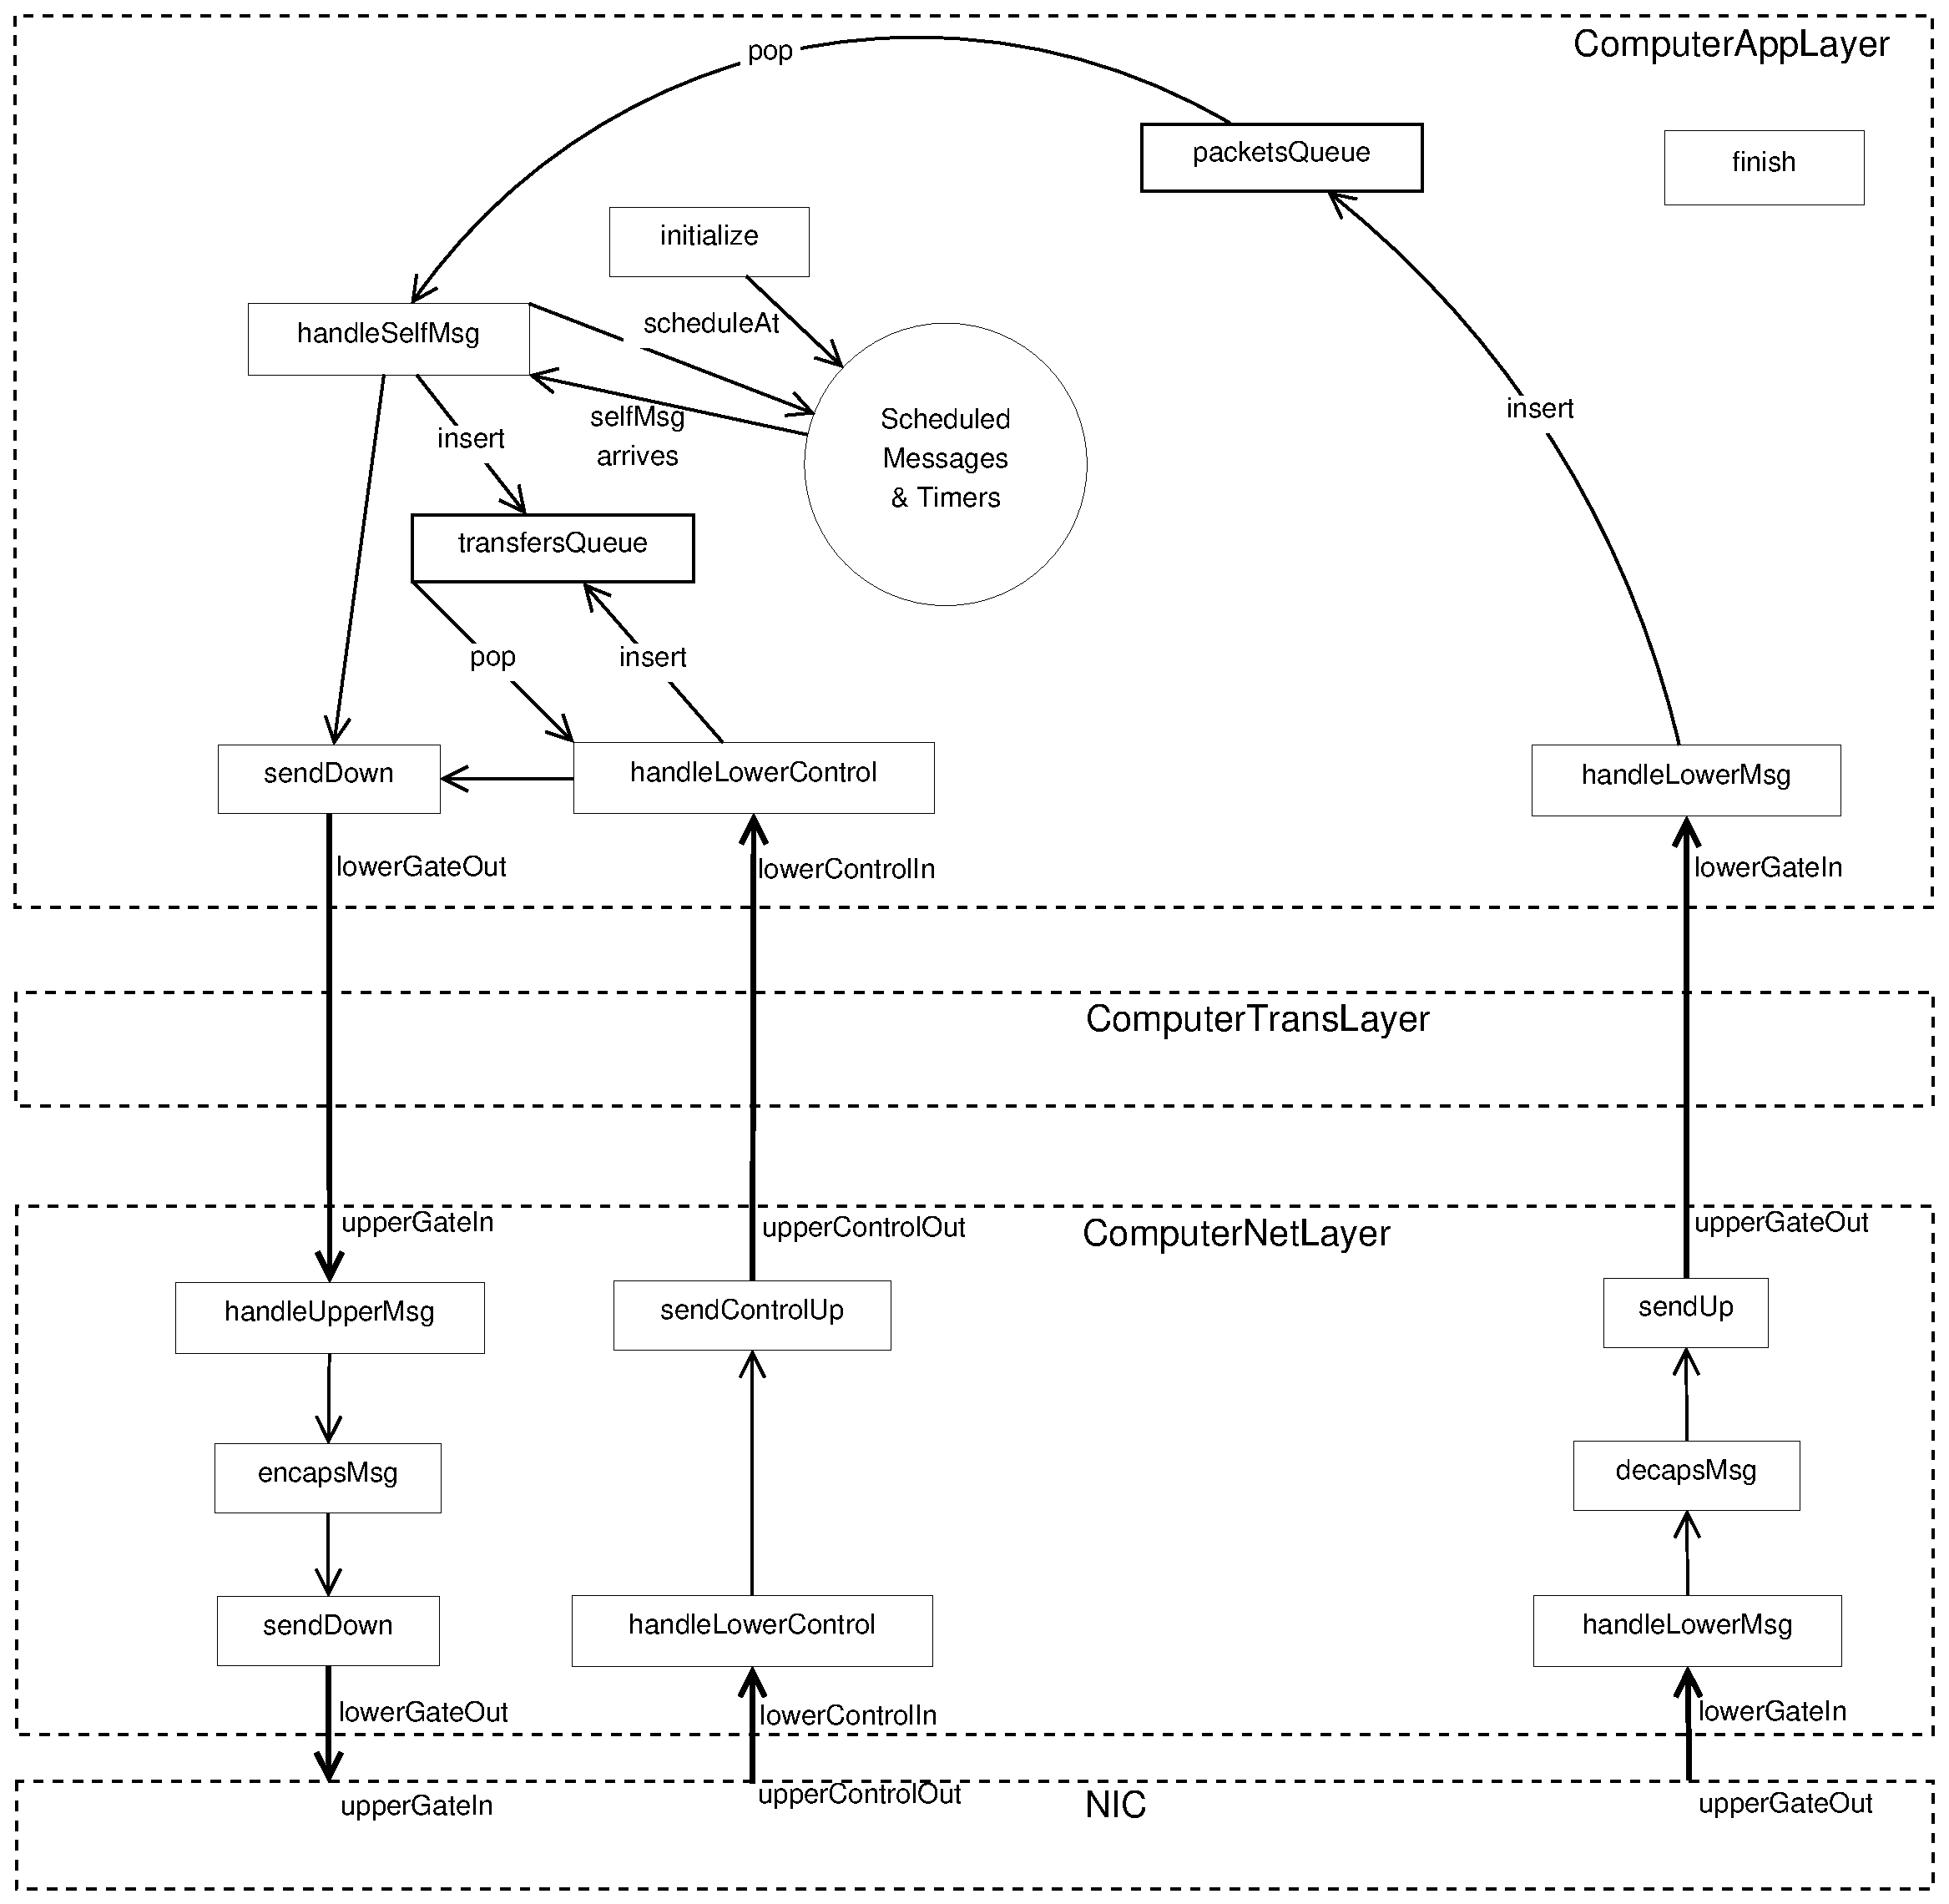
\includegraphics[width=0.9\textwidth]{Computerschema.eps}
  \end{center}
  \caption{Computer functionality diagram}
  \label{fig:Computerschema}
\end{figure}

All methods and elements in the figure will be described next:

\begin{itemize}
  \item \textbf{Scheduled Messages \& Timers}. This element is actually a register where modules can store messages. These messages are associated 
  with the time when the messages should be rescued from the register. Every time that simulation time reaches one of these message's times, the 
  message is recovered from the register and received as self message in the module. This message is handled by \textit{handleSelfMsg} method, 
  which will filter the message according to its kind, in order to decide which action should be carried out. This register is used to program actions in a 
  future time, send messages with delay or just to have timers for any other use. To schedule a new message, the method \textit{scheduleAt} has 
  to be used.
 
  \item \textbf{\textit{initialize}}. In this method, apart from initializing some variables, the Computer calculates the slot distribution among the 
  \acp{AN}. Slot calculation is done at \textit{stage} 3 and according to the algorithm showed in Section \ref{subsec:slottedsyncphase} 
  (\nameref{subsec:slottedsyncphase}). 

  \item \textbf{\textit{finish}}. Records the number of dropped and erased packets due to different reasons as well as the number of packets
  correctly received and sent. It is executed at the end of the simulation.

  \item \textbf{\textit{sendDown}}. This method sends application packets to the \ac{MAC} Layer. These packets will go first through the Transport 
  and Network layers.

  \item \textbf{\textit{transfersQueue}}. This queue was created to store in Application Layer an exact copy of the \ac{MAC} queue. Whenever a packet
  is sent down, a copy is stored in the \textit{transfersQueue}. This way, the packet trying to be sent by \ac{MAC} Layer will be always on the
  first position of the queue. In case the transmission fails or succeeds this will be notified from \ac{MAC} to Application Layer. Method
  \textit{handleLowerControl} will handle this control message acting over the first position in \textit{transfersQueue} in different ways (will 
  be explained later).

  \item \textbf{\textit{packetsQueue}}. Computer can receive only packets from \acp{AN} and never directly from \acp{MN}. The phases where \acp{AN}
  and Computer communicate among them are ComSink 1 and 2. During ComSink Phase 1, the traffic goes in direction to computer (up-links) and, during
  ComSink Phase 2, the traffic goes in direction to selected \acp{AN} (down-links). This means that, during ComSink 1, the Computer only receives messages
  and, during ComSink 2, it only sends messages. Therefore, a queue is needed to store all messages received during ComSink 1 until they are
  transmitted during ComSink 2. This queue is the \textit{packetsQueue}.

  \item \textbf{\textit{handleLowerControl}}. If \ac{MAC} Layer wants to communicate to the Application Layer that some event occurred, it can do 
  it using control messages. Possible control messages were commented in sub-section \ref{sec:macmodifications} (page \pageref{sec:macmodifications}).
  These control messages are handled in Application Layer by this method. Depending on the received control message, the following actions will
  be done by the method:
  \begin{itemize}
    \item[-] \textit{PACKET\_DROPPED\_BACKOFF}. This control message is received when the transmitting packet in the \ac{MAC} Layer was dropped 
    because the maximum number of Backoff tries in \ac{MAC} Layer was reached (\textit{macMaxCSMABackoffs}). If this happens, the method extracts 
    the first message from \textit{transfersQueue} and increases the number of application retries due to Backoff for this message. If the maximum 
    number of retries in the Application Layer is not reached yet, the message is transmitted again (and inserted into the queue) and, if the maximum is 
    reached, the packet is erased. Dropped and erased packets are counted here and recorded with the \textit{finish} method.

    \item[-] \textit{PACKET\_DROPPED}. This control message is received when the transmitting packet in the \ac{MAC} Layer was dropped because
    the maximum number of retransmissions without receiving an \ac{ACK} was reached. If this happens, the method extracts the first message from
    \textit{transfersQueue} and increases the number of application retries due to lack of \ac{ACK} for this message. If the maximum number of 
    retries in application is not yet reached, the message is transmitted again (and inserted into the queue) and, if it is reached, the packet 
    is erased. Dropped and erased packets are counted here and recorded with the \textit{finish} method.

    \item[-] \textit{QUEUE\_FULL}. This control message is received if the last packet which was sent down found the \ac{MAC} Layer queue full. 
    When \ac{MAC} Layer queue is full, it cannot accept more packets and rejects all the received packets, notifying this to the Application Layer. If 
    this happens, the message is removed from the \textit{transfersQueue} and a counter, indicating the number of packets erased due to \ac{MAC} 
    Layer queue full, is increased.

    \item[-] \textit{SYNC\_SENT}. This control message is received when a broadcast was successfully transmitted into the channel. When this happens,
    and to remain \textit{transfersQueue} like a copy of the \ac{MAC} Layer queue, the first element in \textit{transfersQueue} is deleted.

    \item[-] \textit{TX\_OVER}. This control message is received when a report was successfully sent and the \ac{ACK} was also received. When this 
    happens, for the same reason as before, the first element in \textit{transfersQueue} is deleted.

    \item[-] \textit{ACK\_SENT}. This control message is received whenever an \ac{ACK} is sent by the \ac{MAC} Layer. For Computer or \ac{AN} cases 
    is not important, but, this control message is needed for the \acp{MN}.
  \end{itemize}

  \item \textbf{\textit{handleLowerMsg}}. Whenever the Computer receives a packet at its Application Layer, this method is executed. The purpose
  of this method is to handle the different kind of arrived packets according to the phase in which they arrived. For the Computer case, all received packets
  out of the ComSink Phase 1 and coming from a node different to an \ac{AN} are rejected. When a non rejected report is received in the Computer, it 
  will be resent again to the \ac{MN} where it came from (\textit{realSrcAddr}). For this purpose, addresses in the packet are interchanged, setting 
  as \textit{realDestAddr} the address of the \ac{MN} and as \textit{destAddr} the address of the selected \ac{AN}. As the Computer does not send packets
  out of ComSink Phase 2, this packet has to be stored first in its \textit{packetsQueue}.

  \item \textbf{\textit{handleSelfMsg}}. Whenever a self message is received in the Application Layer, it is handled by this method. The following 
  kinds of self messages are processed by this method:
  \begin{itemize}
    \item \textit{CHECK\_QUEUE}. As it was already commented, the Computer can send only packets during ComSink Phase 2 and, therefore, it needs a 
    queue to store the packets to be sent until this phase begins. To check if this queue has still elements to be sent, this self message is programmed.
    Whenever a self message of this type is received, this method checks if there are still elements in the \textit{packetsQueue}. In this case,
    the first element in the queue is sent and a copy stored in the \textit{transfersQueue}. After that, if the \textit{packetsQueue} has still
    packets to be sent, the self message is rescheduled in the next time. The random times when all packets will be sent are calculated at the
    beginning of the ComSink Phase 2.

    \item \textit{BEGIN\_PHASE}. This self message is scheduled at the beginning of every single phase during the simulation. Its task is to 
    configure the phase. The first thing all phases do, is to delete all the messages in the \textit{transfersQueue}. These are the messages for which 
    there was no time in the previous phase. These messages must be deleted to do not interfere in the next phase (in a future work they could be 
    recycled some way). As this queue is a copy of the \ac{MAC} Layer's queue, the same is done in that layer. All phases must also calculate the 
    next phase start time and reschedule the self message at that time.

    Apart from these tasks, at the beginning of ComSink Phase 2, packets to be sent during this phase are going to be handled. At this point, and 
    if the \textit{packetsQueue} has elements, all random transmission times for these packets are calculated. These times are calculated dividing 
    first the ComSink Phase 2 in as much fragments as elements the queue has. Afterwards, a random time is calculated inside each fragment and
    is assigned to each element in the queue. Then, the first element in the queue is prepared to be sent, scheduling the self message 
    \textit{CHECK\_QUEUE}.
  \end{itemize}
\end{itemize}


\subsection{\acp{AN} Application Layer}

The functionality of the \acp{AN} Application Layer is contained in the class \textit{AnchorAppLayer}. The diagram in Figure \ref{fig:ANschema} 
shows a general overview of this functionality together with the Network Layer's one. This class inherits from \textit{AppLayer} class, like
\textit{ComputerAppLayer} did.

\begin{figure}[ht]
 \begin{center}
  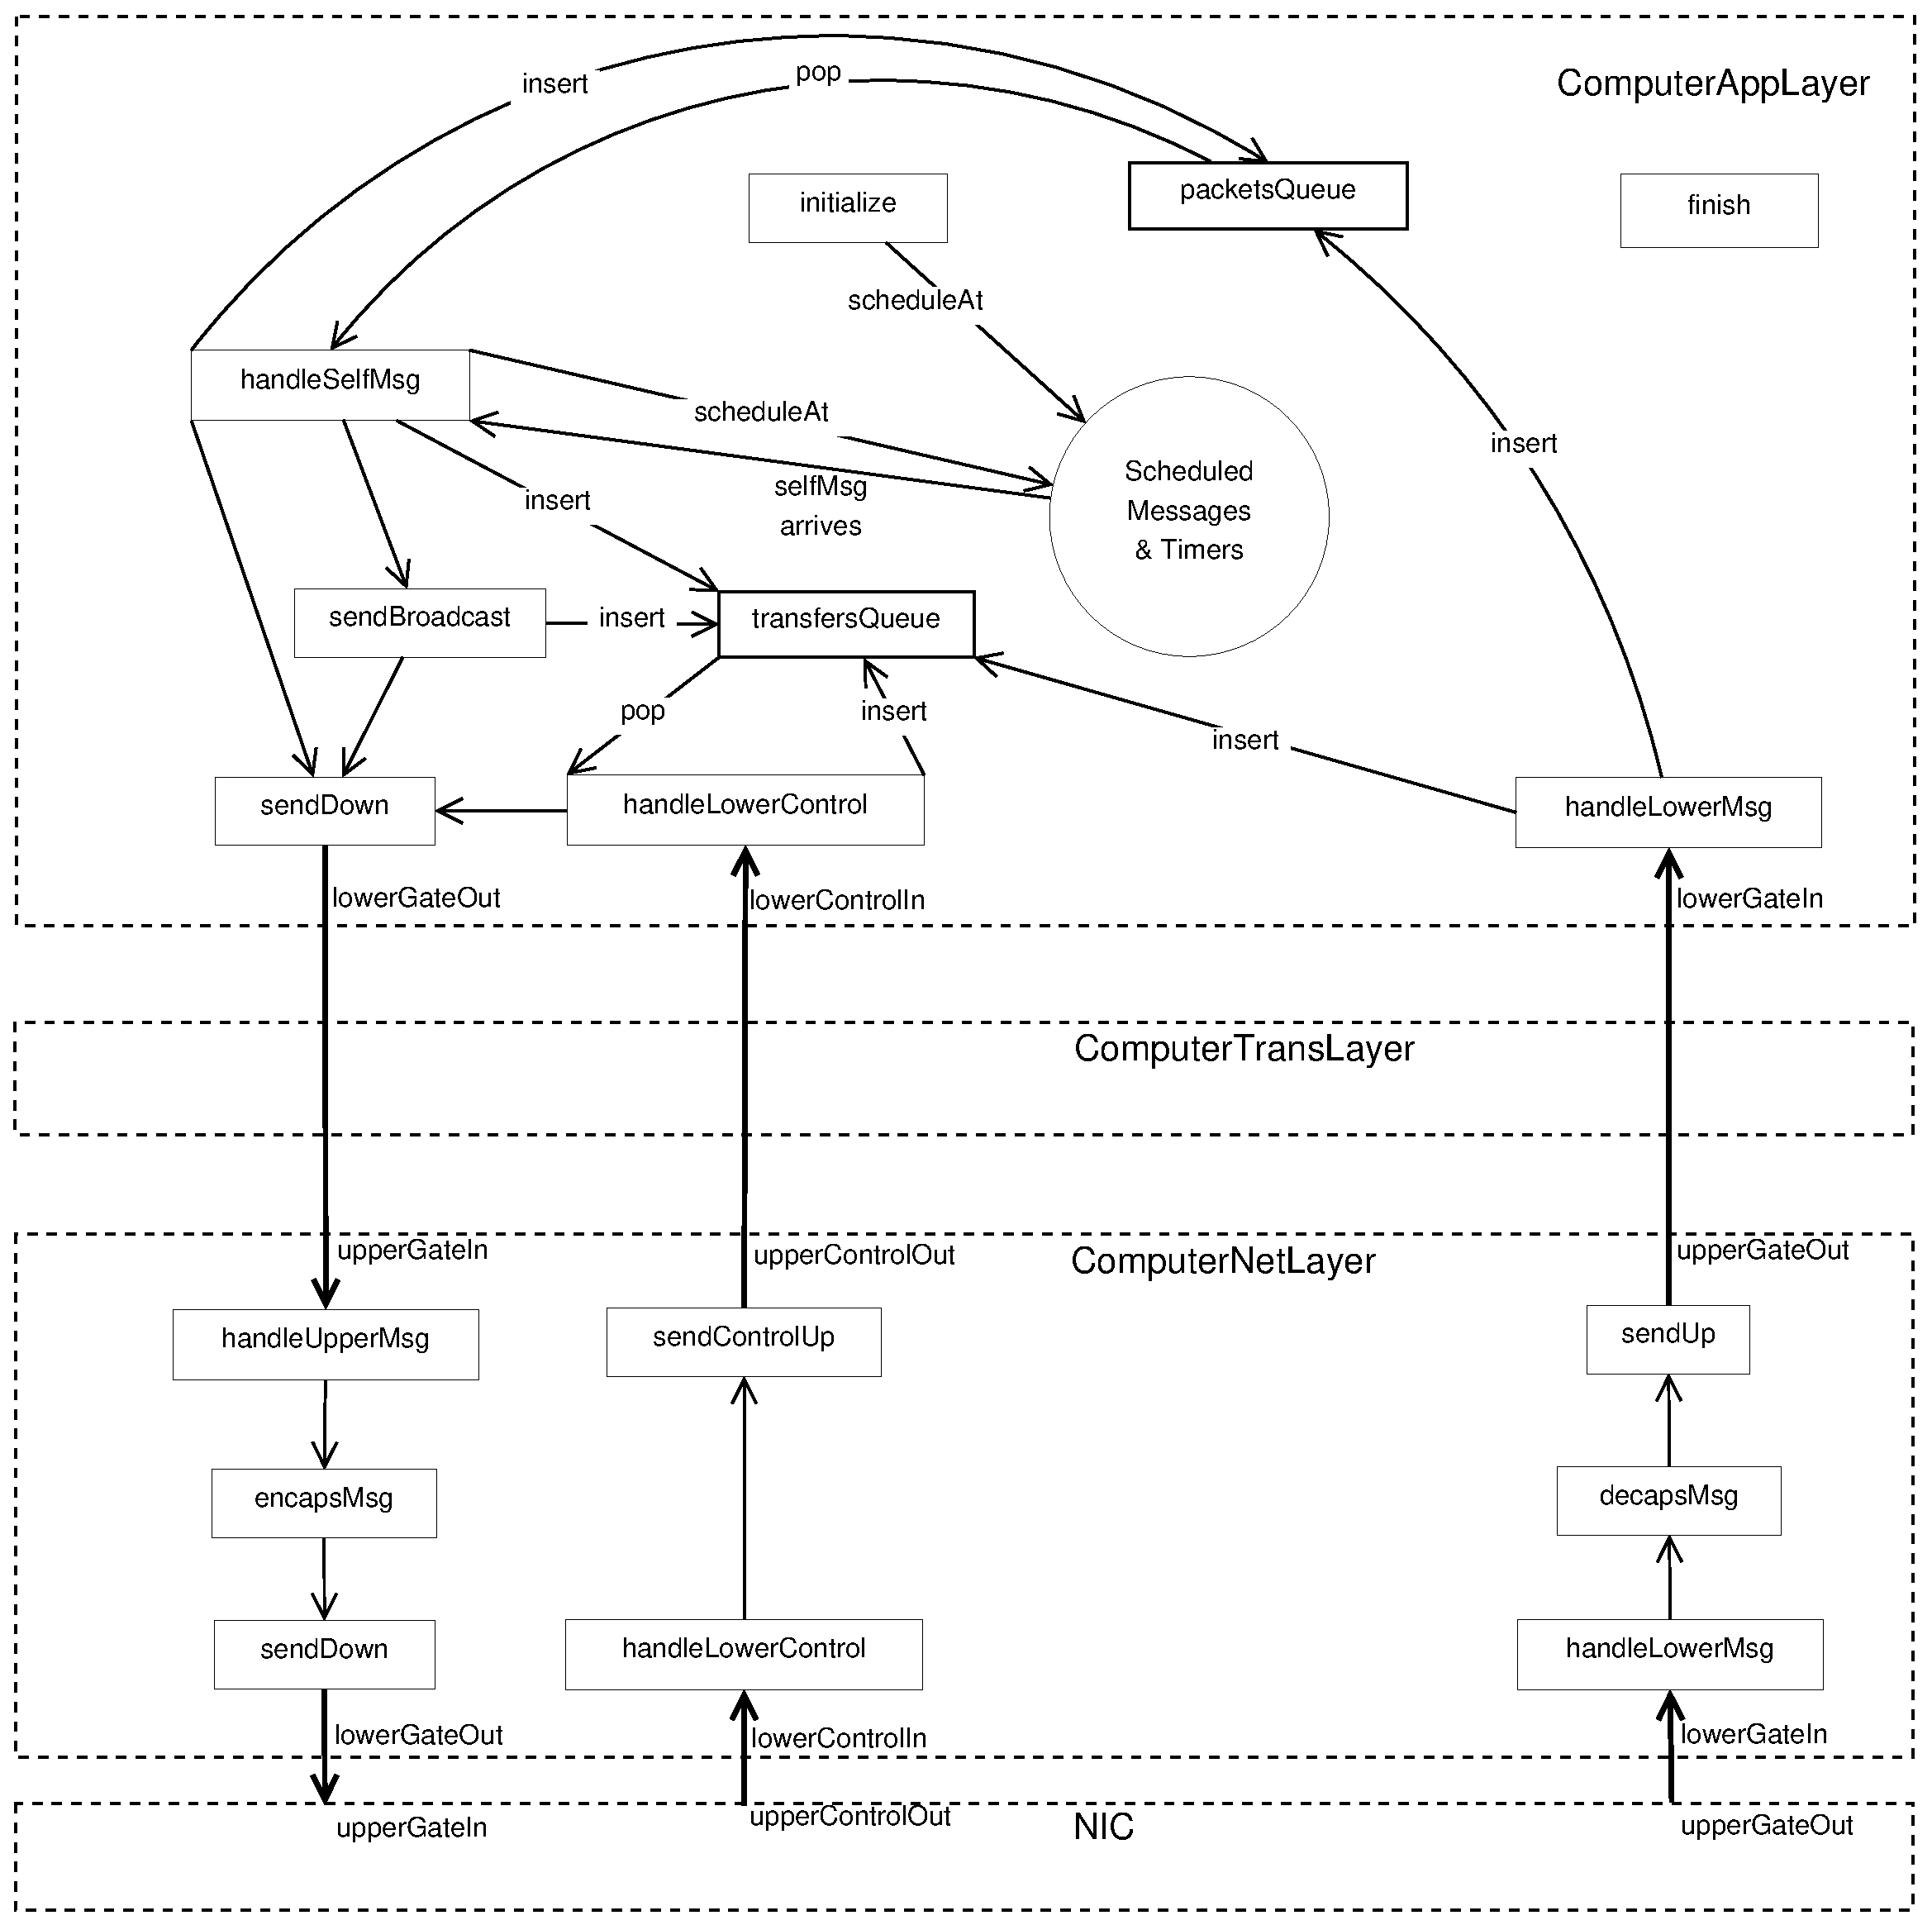
\includegraphics[width=0.9\textwidth]{ANschema.eps}
 \end{center}
 \caption{\acp{AN} functionality diagram}
 \label{fig:ANschema}
\end{figure}

All methods and elements in the figure will be described next:

\begin{itemize}
  \item \textbf{Scheduled Messages \& Timers}. In \acp{AN}, this module works exactly the same as for the Computer. For a deeper explanation, check
  the Computer Application Layer.

  \item \textbf{\textit{initialize}}. This method just initializes some variables.

  \item \textbf{\textit{finish}}. Records the number of dropped and erased packets due to different reasons as well as the number of packets
  correctly received and sent. It is executed at the end of the simulation.

  \item \textbf{\textit{sendDown}}. This method sends application packets to the \ac{MAC} Layer. These packets will go first through the Transport 
  and Network layers.

  \item \textbf{\textit{sendBroadcast}}. This method is called whenever a broadcast wants to be sent; for example, during Sync Phase. Before sending
  the message down, an application message is created and initialized with the correct message type and data. One thing to take into account is that,
  if the broadcast is a sync message to be slotted, \ac{CSMA/CA} must be disabled. This fact is communicated to the \ac{MAC} Layer by means of a 
  variable included in the packet. Remember that a copy must be inserted into the \textit{transfersQueue}.

  \item \textbf{\textit{transfersQueue}}. In \acp{AN}, this module works exactly the same as for the Computer. For a deeper explanation, check
  the Computer Application Layer.

  \item \textbf{\textit{packetsQueue}}. When an \ac{AN} receives a packet from another \ac{AN}, it must be during the ComSink Phases. These packets
  will be routed immediately towards the Computer or the selected \ac{AN}. When an \ac{AN} receives a packet (report or broadcast) from a \ac{MN}, 
  it is during the Report or \ac{VIP} Phases. If this packet is intended to be routed till the Computer (centralized mode), it has to be stored in 
  a queue until it can be sent during the next ComSink Phase 1. This queue is the \textit{packetsQueue}. All this process will be explained better 
  in the following method explanations.

  \item \textbf{\textit{handleLowerControl}}. This method works exactly the same as for the Computer. For a deeper explanation, check the Computer 
  Application Layer.

  \item \textbf{\textit{handleLowerMsg}}. Whenever an \ac{AN} receives a packet at its Application Layer, this method is executed. The purpose
  of this method is handling the different kind of arrived packets according to the phase when they arrived. The following situations are possible:
  \begin{itemize}
    \item Report received from a \ac{MN} during Report Phase. There are three types of reports which can be received during this phase:
    \begin{itemize}
      \item Request packet. In this case, an answer is sent immediately to the \ac{MN}. A copy of this is inserted in the \textit{transfersQueue}.

      \item Report in Distributed-A mode. This report provides some information to the \ac{AN}. Right now, the packet is just deleted. In future
      works, it could be saved or processed some other way.

      \item Report in Centralized mode. This report has to be routed until the Computer but, as this will be done in ComSink Phase 1, first it is
      inserted in \textit{packetsQueue}.
    \end{itemize}

    \item Broadcast received from a \ac{MN} during Report or \ac{VIP} Phases. This broadcast is saved together with all the broadcasts received
    from the same \ac{MN}. At the beginning of Sync Phase 2, it is generated a report for each \ac{MN} from which the \ac{AN} received at least one 
    broadcast. This report contains the address of the \ac{MN} and an average of all the \ac{RSSI} values got from all the received broadcasts.

    \item Report received from an \ac{AN} or the Computer during a ComSink Phase. In this case there are also three types of reports which can be 
    received during this phase:
    \begin{itemize}
      \item Report to be routed. This report is not for this \ac{AN} and is just sent down and inserted in \textit{transfersQueue}.
      
      \item Report for this \ac{AN}. This report is now deleted but, in future works, it could be used by the Computer to communicate with 
      the \acp{AN}.

      \item Report for a \ac{MN}. This report is for a \ac{MN} to which this \ac{AN} is the selected \ac{AN}. This packet was probably requested
      from the \ac{MN}. In future works, this packet would be saved and sent to the \ac{MN} when requested. Right now is just deleted.
    \end{itemize}
  \end{itemize}

  \item \textbf{\textit{handleSelfMsg}}. Whenever a self message is received in the Application Layer, it is handled by this method. The 
  following kinds of self messages are processed by this method:
  \begin{itemize}
    \item \textit{SEND\_SYNC\_TIMER\_WITHOUT\_CSMA}. When this self message is received, \textit{sendBroadcast} method is called to send 
    a broadcast. In this case the broadcasts are sync messages. The time to transmit the next sync message is also calculated according 
    to the assigned slots for each \ac{AN} and to the number of sub phases in the Sync Phase.

    \item \textit{CHECK\_QUEUE}. As it was already commented, any time an \ac{AN} receives or generates a message to be sent to the Computer 
    out of the ComSink Phase 1, this message is saved in \textit{packetsQueue} waiting to be sent. To check if this queue has still elements 
    to be sent, this self message is programmed. Whenever a self message of this type is received, this method checks if there are still 
    elements in the \textit{packetsQueue}. In this case, the first element in the queue is sent and a copy stored in the \textit{transfersQueue}.
    After that, if the \textit{packetsQueue} has still packets to be sent, the self message is rescheduled in the next time. The random times 
    when all packets will be sent are calculated at the beginning of the ComSink Phase 1.

    \item \textit{BEGIN\_PHASE}. This self message is scheduled at the beginning of every single phase during the simulation. Its task is to 
    configure the phase. The first thing all phases do is deleting all messages in the \textit{transfersQueue}. These are the messages for which 
    there was no time in the previous phase. These messages must be deleted not to interfere in the next phase (in a future work they could be 
    recycled some way). As this queue is a copy of the \ac{MAC} Layer's queue, the same is done in that layer. All phases must also calculate the 
    next phase start time and reschedule the self message at that time. Apart from these tasks, some phases have their own jobs to be done:
    \begin{itemize}
      \item \textit{SYNC\_PHASE\_1}. At the beginning of this phase, the first sync message of this phase will be scheduled using the 
      already seen self message.

      \item \textit{SYNC\_PHASE\_2}. As it was already seen, at the beginning of this phase, it is generated a report for each \ac{MN} from which 
      the \ac{AN} received at least a broadcast. This report contains the address of the \ac{MN} and an average of all the \ac{RSSI} values 
      got from all the received broadcasts. This report is then inserted into the \textit{packetsQueue} to be transmitted during ComSink Phase 1.
      
      At the beginning of this phase, the first sync message of this phase will be scheduled like for \textit{SYNC\_PHASE\_1}.

      \item \textit{COM\_SINK\_PHASE\_1}. At the beginning of this phase, packets to be sent during this phase are going to be handled. At 
      this point, and if the \textit{packetsQueue} has elements, all random transmission times for these packets are calculated. These times 
      are calculated dividing first the ComSink Phase 1 in as much fragments as elements the queue has. Afterwards, a random time is 
      calculated inside each fragment and assigned to each element in the queue. Then, the first element in the queue is prepared to be 
      sent, scheduling the self message \textit{CHECK\_QUEUE}.

      \item \textit{SYNC\_PHASE\_3}. At the beginning of this phase, the first sync message of this phase will be scheduled like 
      for \textit{SYNC\_PHASE\_1}.
    \end{itemize}
  \end{itemize}
\end{itemize}


\subsection{\acp{MN} Application Layer}

The functionality of the \acp{MN} Application Layer is contained in the class \textit{NodeAppLayer}. The diagram in Figure \ref{fig:MNschema} 
shows a general overview of this functionality together with the Network Layer's one. This class inherits from \textit{AppLayer} class, like
\textit{ComputerAppLayer} did.

\begin{figure}[ht]
 \begin{center}
  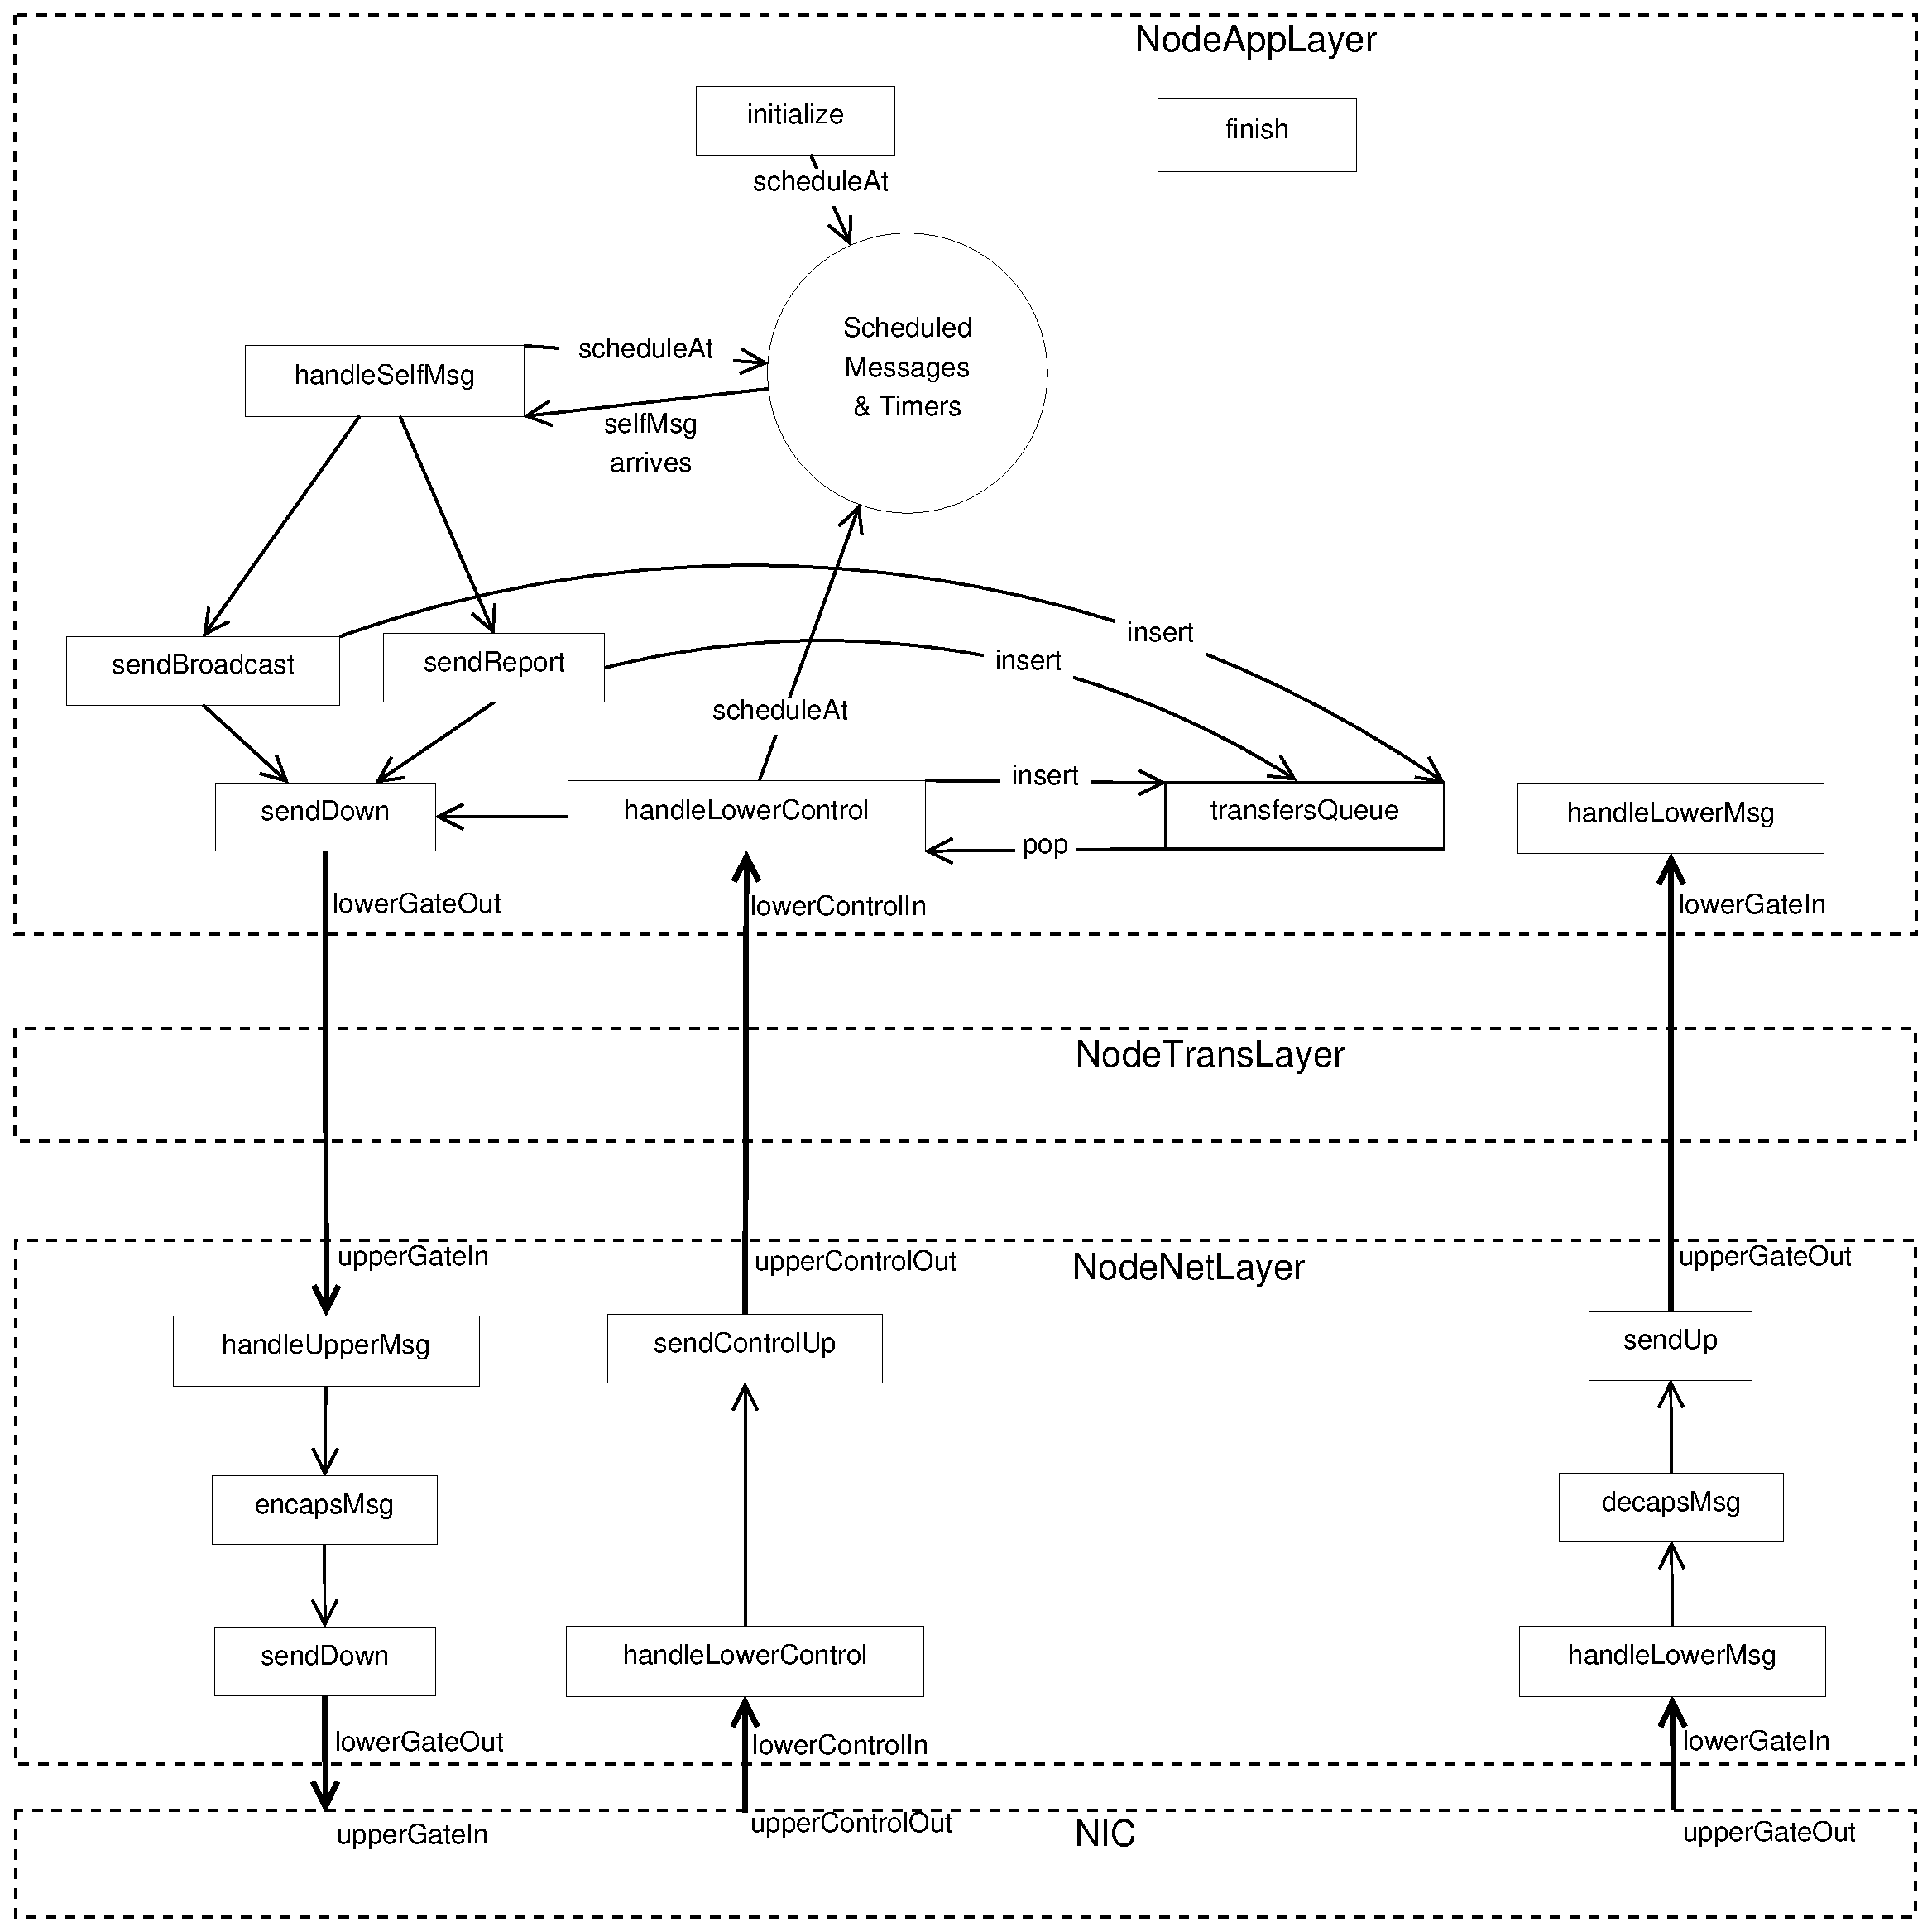
\includegraphics[width=0.9\textwidth]{MNschema.eps}
 \end{center}
 \caption{\acp{MN} functionality diagram}
 \label{fig:MNschema}
\end{figure}

All methods and elements in the figure will be described next:

\begin{itemize}
  \item \textbf{Scheduled Messages \& Timers}. In \acp{MN}, this module works exactly the same as for the Computer. For a deeper explanation, check
  the Computer Application Layer.

  \item \textbf{\textit{initialize}}. This method just initializes some variables.

  \item \textbf{\textit{finish}}. Records the number of dropped and erased packets due to different reasons as well as the number of packets
  correctly received and sent. It is executed at the end of the simulation.

  \item \textbf{\textit{sendDown}}. This method sends application packets to the \ac{MAC} Layer. These packets will go first through the Transport 
  and Network layers.

  \item \textbf{\textit{sendBroadcast}}. This method is called whenever a broadcast wants to be sent, and always during Report or \ac{VIP} Phases. 
  Before sending the message down, an application message is created and initialized with the correct message type and data. Unlike for the \acp{AN},
  here \ac{CSMA/CA} must remain active. Remember that a copy must be inserted into the \textit{transfersQueue}.

  \item \textbf{\textit{sendReport}}. \ac{MN}'s reports are just sent to selected \acp{AN}. That is why, before sending them, it is always needed
  to listen to Sync Phase 1 to find which \ac{AN} is the selected \ac{AN}. When sync packets are received, a \ac{RSSI} list is created. Before 
  doing anything else, \textit{sendReport} method checks this list to assign the destination address. In the case the \ac{RSSI} list is empty, an 
  error will notify of this fact. After assigning the destination address, the real destination address is assigned. This address will be 
  the Computer's address if the \ac{MN} is working in centralized mode and the selected \ac{AN} address in the case the \ac{MN} is working in 
  Distributed-A mode.

  Next thing to do is to assign the packet size in order to model the real packet behavior. Depending on the type of report to be sent, different 
  sizes will be chosen. A complete list of this types was already explained in sub-section \ref{sec:packetstructure} (page 
  \pageref{sec:packetstructure}).

  A last detail must be taken into account before sending the packet down. For the case in which the \ac{MN} wants to ask for some information, the 
  ASK flag will be activated in the packet and the address of the selected \ac{AN} saved. This address is saved because, in case the \ac{MN} moves 
  and its selected \ac{AN} changes, the \ac{MN} will still need to ask for the information to the first \ac{AN}. This \ac{AN} will be the one 
  having the information ready to be requested and not the new selected \ac{AN}. For the case in which the \ac{MN} wants to request the previously 
  asked information, the Request flag will be activated in the packet. As it was said, the destination address to be used in this case is the 
  one saved by the \ac{MN} when asking for information.

  Now the packet is ready to be sent down, but not before saving a copy in the \textit{transfersQueue}.

  \item \textbf{\textit{transfersQueue}}. In \acp{MN}, this module works exactly the same as for the Computer. For a deeper explanation, check
  the Computer Application Layer.

  \item \textbf{\textit{handleLowerControl}}. The basic functionality of this method is exactly the same as for the Computer. For a deeper explanation, 
  check the Computer Application Layer. The main difference between this method and the one for the Computer is that this method decides in which 
  situations, when receiving a control message, the \ac{MN} is allowed to sleep or must remain awake. All these cases will be explained at the end of this
  section, together with the ones from all the other methods.

  \item \textbf{\textit{handleLowerMsg}}. Whenever a \ac{MN} receives a packet at its Application Layer, this method is executed. The purpose
  of this method is handling the different kind of arrived packets according to the phase when they arrived. The following situations are possible:
  \begin{itemize}
    \item Broadcast received during a Sync Phase. The \acp{MN} listen to these broadcasts to get \ac{RSSI} samples and get synchronized. For this 
    case, this method makes a list with all the \ac{RSSI} values received per \ac{AN}. This list will be used by the \textit{sendReport} method to 
    decide which \ac{AN} is the selected \ac{AN}.

    \item Reports from selected \ac{AN}, received during a Report Phase, which are answering a request. In this case, the method will record if the packet was
    received during the waiting time left for this purpose, or out of it. If it was received in the suitable moment, the timer will be canceled to
    avoid idle listening in the \ac{MN}.
  \end{itemize}

  \item \textbf{\textit{handleSelfMsg}}. Whenever a self message is received in the Application Layer, it is handled by this method. The following 
  kinds of self messages are processed by this method:
  \begin{itemize}
    \item \textit{SLEEP}. It will be explained at the end of this section.

    \item \textit{WAKE\_UP}. It will be explained at the end of this section.

    \item \textit{SEND\_REPORT\_WITH\_CSMA}. In this case, the method will check if the \ac{MN} is already calculating its own position (only for 
    \acp{MN} in Mode 2). In this case, the self message will be rescheduled a random time after the calculation process. If the \ac{MN} 
    was not busy, \textit{sendReport} method will be called.

    \item \textit{SEND\_SYNC\_TIMER\_WITH\_CSMA}. In this case, \textit{sendBroadcast} method is called to send a broadcast. If there are still 
    more broadcasts to send, the self message is rescheduled a time later. The times when the broadcasts are going to be sent are calculated 
    by the method \textit{createRandomBroadcastTimes}.

    \item \textit{CALCULATE\_POSITION}. When this self message is received, there are two options. If the \ac{MN} was calculating its position, then
    the timer is ended and the energy status updated. If the \ac{MN} was not still calculating its position, a new timer is started scheduling its end
    some processing time later (\textit{processingTime}). The \ac{MN}'s position is also stored in a list to be sent with an extra report.

    \item \textit{WAITING\_REQUEST}. When a request is correctly transmitted, method \textit{handleLowerControl} starts a waiting time timer. If the
    self message due to this timer is received, it means that no \ac{AN}'s answer was received on time. This method restarts then all waiting time 
    variables to its default values and records this situation.

    This self message is also used to schedule a request packet. When a \ac{MN} wants to perform a request, Application Layer schedules a 
    \textit{WAITING\_REQUEST} self message at the middle of Sync Phase 1. The reason to schedule the self message at that time is because there all 
    reports or extra reports are already scheduled and can be found. When this self message is handled, the first thing to do is to look if a 
    report or extra report is already scheduled. If this is the case, the request flag could be activated in it. If not, a new extra report is 
    created and scheduled.

    The request process provides information to the \ac{MN}, probably for a configuration change or a position. This process is, hence, really 
    important and must be given a higher priority. That is why, when a \ac{MN} in Mode 4 makes a request, its broadcasts are canceled 
    to reduce the traffic during the Report Phase, arising this way the probability of a successful delivery of the request packet and its
    answer.

    To distinguish between these two cases, the variable \textit{waitForAnchor} is used. If the value is 0, the method will schedule a request
    and, if not, the waiting time timer will be handled (in this case \textit{waitForAnchor} will take as value the address of the \ac{AN} from
    which the answer is expected).

    \item \textit{BEGIN\_PHASE}. This self message is scheduled at the beginning of every single phase during the simulation. Its task is to 
    configure the phase itself and, in some cases, also the whole period (beginning of Sync Phase 1). Regardless of the phase, the first thing to
    do is deleting all messages in the \textit{transfersQueue}. These are the messages for which there was no time in the previous phase. These 
    messages must be deleted to do not interfere in the next phase (in a future work they could be recycled some way). As this queue is a copy of the
    \ac{MAC} Layer queue, the same is done in that layer. Another task, that all phases have in common, is to calculate the next phase start time
    and rescheduling the self message at that time. This is done just after the \textit{transfersQueue} is emptied. From this point, the actions
    to carry out will depend on the phase the node is in:
    \begin{itemize}
      \item \textit{SYNC\_PHASE\_1}. At the beginning of this phase, not only this phase will be configured but also some aspects for the whole
      period. The tasks to be done at this point are:
      \begin{itemize}
	\item If the period is active, the Sync Phase is not affected by the Sync Phase Offset. For a \ac{MN} which is not in Mode 3, this Sync Phase will
	be enabled to be listened to.

	\item The \ac{RSSI} list is cleaned. This way the old values will not interfere with the new ones to be listened to.

	\item Reports for \acp{MN} in Modes 1 and 4 are going to be scheduled if the active period is the last one of the collection.

	\item If \ac{MN} is in Mode 2 and the active period is the last one of the collection, the timer for calculating the \ac{MN}'s position will 
	be started.

	\item If \ac{MN} is in Mode 3 or 4, the broadcast's random transmitting times are going to be calculated. This is done with the method 
	\textit{createRandomBroadcastTimes}. This method assigns a random time to every broadcast to be transmitted and leaves a minimum time
	distance among all generated times. In case the \ac{MN} is in Mode 4 and, during this period, an extra report is also scheduled, the minimum 
	time distance must also be left within the extra report. At this moment, the first broadcast is also scheduled. If the \ac{MN} is in Mode 3
	and, during this period, an extra report is also scheduled, broadcasts are going to be canceled to save battery, as this report will already
	carry \ac{RSSI} information from the \ac{MN}.

	\item If according to the \ac{MN}'s configuration parameters, there should be scheduled an extra report during this period, it is scheduled at 
	this moment. The first thing to do is enabling Sync Phase 1 to be listened to in case it was not enabled. Before scheduling a new extra report, it has 
	to be checked if another report is already scheduled. If this happens, the extra report will not be scheduled and the normal report will 
	be used.

	Every time an extra report is sent, a counter is increased. When this counter reaches the value of the parameter \textit{askFrequency}, 
	the extra report gets the ASK flag activated and a request packet is scheduled for the next period as it was already told.
      \end{itemize}

      \item \textit{REPORT\_PHASE}. At this point just the sleep and wake up management will be done. As it was said, all cases will be explained 
      together at the end of the section.

      \item \textit{VIP\_PHASE}. At this point just the sleep and wake up management will be done. As it was said, all cases will be explained 
      together at the end of the section.

      \item \textit{SYNC\_PHASE\_2}. If \ac{MN} is not in Mode 3 and the period is active, this Sync Phase will be enabled to be listened to. However,
      there are two exceptions in which this phase will not be enabled. One is when the active period is the last one in the active periods collection. 
      The other is when the active period is the first and this Sync Phase is affected by the Sync Phase Offset.

      \item \textit{COM\_SINK\_PHASE\_1}. At this point just the sleep and wake up management will be done. As it was said, all cases will be 
      explained together at the end of the section.

      \item \textit{SYNC\_PHASE\_3}. If \ac{MN} is not in Mode 3 and the period is active, this Sync Phase will be enabled to be listened to. However,
      when the active period is the last one in the active periods collection, this phase will not be enabled.

      \item \textit{COM\_SINK\_PHASE\_2}. At this point just the sleep and wake up management will be done. As it was said, all cases will be 
      explained together at the end of the section.

    \end{itemize}
  \end{itemize}
\end{itemize}

A last detail to be studied and probably the most important for the \ac{MN} is, when are the nodes going to sleep and when should they wake up? 
Even though Sleep and Wake-Up transitions are done during the previously explained methods, they are explained next and all together for a 
better understanding.

A transition between SLEEP state and any other takes some time (durations can be seen in source code in class \textit{EnergyConsumption}). That is why,
before sleeping a node, it has to be checked if some other event, where the node must be awake, is coming sooner than the time needed to sleep and
wake up the node again (from now on, T). Consequently, it is deduced, that the \ac{MN} can go to sleep in the following situations:

\begin{itemize}
 \item Always at the beginning of ComSink 1 and 2 (Done in \textit{handleSelfMsg} method).
 
 \item At the beginning of Sync Phases in \underline{any} of the following cases (Done in \textit{handleSelfMsg} method):
    \begin{itemize}
      \item[-] Inactive periods.
      \item[-] First offset periods.
      \item[-] Second and third Sync Phases in last active period.
      \item[-] Sync Phases affected by the Sync Phases offset.
      \item[-] If \ac{MN} is in Mode 3.
      \item[-] If there are no active periods.
    \end{itemize}
  The only exception to this, where \ac{MN} cannot go to sleep, is when an extra report is scheduled. In this case it does not matter if the 
  previous conditions are fulfilled or not. At the beginning of the first Sync Phase in this period, the \ac{MN} must be awake.

 \item At the beginning of \ac{VIP} Phase if next broadcast is scheduled in a time bigger than T (Done in \textit{handleSelfMsg} method).

 \item At the beginning of a Report Phase if \underline{all} these conditions get fulfilled (Done in \textit{handleSelfMsg} method):
    \begin{itemize}
      \item[-] Next extra report comes after T.
      \item[-] Next report comes after T.
      \item[-] Next broadcast comes after T (just for \ac{MN} in Mode 4).
    \end{itemize}

  \item When a report was successfully sent, if the \textit{transfersQueue} has no elements and \underline{all} these conditions get fulfilled 
  (Done in \textit{handleLowerControl} method):
    \begin{itemize}
      \item[-] Next broadcast comes after T (just for \ac{MN} in Mode 4).
      \item[-] The report was not a request. In this case, instead of sleeping the \ac{MN}, a timer to wait for the \ac{AN}'s answer is started.
    \end{itemize}

  \item When erasing a report due to maximum number of retries, if the \textit{transfersQueue} has no elements and if next broadcast (just for 
  \ac{MN} in Mode 4) comes after T (Done in \textit{handleLowerControl} method).

  \item When a broadcast was successfully sent into the channel, if the \textit{transfersQueue} has no elements and \underline{all} these 
  conditions get fulfilled (Done in \textit{handleLowerControl} method):
    \begin{itemize}
      \item[-] Next broadcast comes after T.
      \item[-] Next report comes after T (just for \ac{MN} in Mode 4).
      \item[-] Sync Phase 2 begins after T (just for \ac{MN} in Mode 3).
    \end{itemize}

  \item When erasing a broadcast due to maximum number of retries, if the \textit{transfersQueue} has no elements and \underline{all} these 
  conditions get fulfilled (Done in \textit{handleLowerControl} method):
    \begin{itemize}
      \item[-] Next broadcast comes after T.
      \item[-] Next report comes after T (just for \ac{MN} in Mode 4).
      \item[-] Sync Phase 2 begins after T (just for \ac{MN} in Mode 3).
    \end{itemize}

  \item When the waiting time timer in request process ended, if the \textit{transfersQueue} has no elements and if next broadcast (just for \ac{MN} in 
  Modes 3 and 4) comes after T (Done in \textit{handleSelfMsg} method).

  \item When an answer from an \ac{AN} to a request is received and the \ac{ACK} is sent, if the \textit{transfers\-Queue} has no elements and 
  if next broadcast (just for \ac{MN} in Modes 3 and 4) comes after T (Done in \textit{handleLowerControl} method).
\end{itemize}

To wake up the node, and like for the previous case, transition times between SLEEP state and any other state have to be taken into account. That 
is why, if the \ac{MN} must be awake for a certain event, it is important to wake it up some time before this event is coming. This time must be 
at least the time needed by \ac{MN} to go from SLEEP state to \ac{Rx} state (from now on, $T_2$). \ac{MN} must wake up in the following situations:

\begin{itemize}
  \item A time $T_2$ before the start of each Sync Phase if \underline{all} these conditions are fulfilled (Done in \textit{handleSelfMsg} method):
    \begin{itemize}
      \item[-] \ac{MN} is not in Mode 3.
      \item[-] The period is active.
      \item[-] The Sync Phase is not affected by Sync Phase Offset.
      \item[-] The Sync Phase is not the second or third Sync Phases in the last active period.
    \end{itemize}
  
  \item A time $T_2$ before the start of Sync Phase 1 if there is an extra report scheduled in this period (Done in \textit{handleSelfMsg} method).
  
  \item A time $T_2$ before a report is going to be sent.

  \item A time $T_2$ before an extra report is going to be sent.

  \item A time $T_2$ before a broadcast is going to be sent.
\end{itemize}

It is important to remember that any time a report, extra report or broadcast gets canceled, the scheduled wake up order must be also canceled 
or the \ac{MN} will wake up for nothing.

Both actions, sleeping and waking up the \ac{MN}, are called with the methods \textit{goToSleep} and \textit{goToWakeUp} respectively. Whenever
one of these two methods is called, it adds to an array a new time when the \ac{MN} should sleep or wake up. These arrays are then ordered to 
start with the times coming first, and then a self message is scheduled for each array's first element. This self message will be handled by the 
\textit{handleSelfMsg} method, carrying out the following steps:
\begin{itemize}
 \item[-] Sleep or wake up the Radio changing its state to SLEEP or \ac{Rx}.
 
 \item[-] Update the Energy module status calling the \textit{updateStateStatus} method from \textit{EnergyConsumption} class.

 \item[-] Remove the already handled time from the array.

 \item[-] Schedule the next time if there are still times to schedule.
\end{itemize}



